% =====================================================================
%  Auditing the Evaluator — NeurIPS Evaluations & Datasets (E&D) submission (anonymous)
%  v1.4 (689 reframed): STRUCTURAL REFRAME, not a title swap. The paper no longer
%      claims that a failure-driven evolution operator improves verification recall;
%      it asks whether evaluation results survive an audit of the evaluator.
%      - Title: "Evolving Verifiers: ..." -> "Auditing the Evaluator: ..." (evidence
%        does not support the old framing; the negative result becomes Finding 5).
%      - Contributions: 4 (incl. evolution + submodular formalization) -> 3
%        (audit protocol / empirical audit / quantitative findings).
%      - New section 3: Evaluator-Audit Protocol (claim declaration, eight failure
%        modes, falsification procedure, four audit outcomes) -- the transferable core.
%      - Findings reorganised as five audited hypotheses (F1..F5); +24.0pp is presented
%        as a measurement-pool composition artifact, not a win.
%      - Statistics added (689): TOST equivalence test (margin +/-10pp FAILS; 90% CI
%        [-10.61,+5.52]pp; min passing margin 10.61pp), two-way standardization
%        (forward diff -17.92pp; overall-rate similarity is composition offset),
%        three-component environment metrics (catch/unknown/conditional recall).
%      - Hard fixes (689): kd/n -> k*|D|/|A| (see Appendix~\ref{app:noise687});
%        placeholder markers removed (A0-A4 marked "not run"); 18/70 -> 13/34; "Verifier Coverage 73.8%" and
%        "1.9pp/rule" deleted; static arm renamed a calibration arm; kappa values are
%        labelled AI self-consistency (never human IAA); Merkle claims restated as
%        tamper-evident current-state integrity with a threat model; E9 restated as a
%        cross-regime observational comparison; template footer placeholder overridden
%        in this file (the .sty itself is third-party and untouched).
%      - Human annotation: protocol + de-identified package prepared (Appendix~\ref{app:reframe689});
%        execution is PENDING; no human IAA is claimed.
%  v1.3 (677d): paper-merge batch (A5 side-by-side +24.0pp / +7-12pp; cluster bootstrap).
%  v1.2 (677a): framing revision + engineering cleanup.
%  v1.1 (673c): red-team critique revisions + humanization. ALL NUMBERS IDENTICAL TO v1.0.
%  v1.0 (673a): all numbers synced to the authoritative numbers artifact (schema 672h).
%  Engine: tectonic (XeTeX) / pdflatex+bibtex.
%  Template: official neurips_2025.sty -- PLACEHOLDER. We target the NeurIPS 2027
%  Evaluations & Datasets (E&D) track (renamed from Datasets & Benchmarks in 2026).
%  The 2027 CFP is not published; this draft will migrate to the 2027 E&D style upon
%  release. Do NOT edit neurips_2025.sty (third-party file); its default notice string
%  is overridden below with a neutral "under review" placeholder.
% =====================================================================
\documentclass{article}

\usepackage[dandb]{neurips_2025}   % Datasets & Benchmarks track; anonymous by default
\usepackage[utf8]{inputenc}
\usepackage[T1]{fontenc}
\usepackage{hyperref}
\usepackage{url}
\usepackage{booktabs}
\usepackage{amsfonts}
\usepackage{amsmath}
\usepackage{amssymb}
\usepackage{graphicx}
\usepackage{xcolor}
\usepackage{tikz}
\usepackage{pgfplots}
\pgfplotsset{compat=1.17}
\usetikzlibrary{arrows.meta,positioning,shapes.geometric,fit,backgrounds}

\newcommand{\cmark}{\textcolor{green!60!black}{\checkmark}}

% Neutral notice string (the 2027 CFP is unpublished; do not print a wrong year).
\makeatletter
\renewcommand{\@noticestring}{%
  Under review (anonymized). Do not distribute.%
}
\makeatother

\title{Auditing the Evaluator: Stress-Testing\\ Evidence-Based Software Verification}

\author{%
  Anonymous Author(s) \\
  Affiliation \\
  Address \\
  \texttt{email} \\
}

\begin{document}
\maketitle

\begin{abstract}
How often can an apparently convincing evaluation result survive an audit of the evaluator
that produced it? We study a software-verification apparatus---eight evidence-acquisition
assets (sanitizers, compiler warnings, cross-compilation, linker) over C++ assertions---and
show that evaluator claims can materially weaken or collapse under controls that change no
malicious behavior: calibers drift, degenerate assets inflate gains, environments silently
change the instrument, labels move the measured object. We present \textbf{Queyi}, an
executable evaluator-audit protocol: every claim declares its caliber (dataset, asset,
environment, configuration, protocol); eight failure modes structure the audit; claims are
re-measured under adversarial controls and receive one of four outcomes (survives, weakened,
collapses, unresolved). Auditing 1147 self-authored and 110 source-derived CVE-reconstruction
samples yields five findings. (1)~A $+24.0$pp selection gain is mostly measurement-pool
composition: removing degenerate assets leaves $+7.4$--$11.3$pp. (2)~The instrument is blind
to 38.4\% of samples in a family-structured way; 41.5\% of real-defect catches ride on one
asset. (3)~Without the declared WSL profile, real-defect detection falls
59.09\%$\to$23.64\% with \emph{no} unknown increase and no warning---environment is part of
the measurement. (4)~Synthetic and source-derived corpora fail TOST equivalence at $\pm10$pp
(90\% CI $[-10.61,+5.52]$pp); standardization shows the similar headline rates hide a
$-17.9$pp composition offset. (5)~Failure-driven evolution yields no measurable recall gain
over frequency selection (identical selections in 14/14 tier checks; $p{=}0.302$)---an audit
finding, not a contribution. Human annotation is designed but \emph{not executed}; all
$\kappa$ values are AI self-consistency only.
\end{abstract}

% =====================================================================
\section{Introduction}
\label{sec:intro}
% =====================================================================
\paragraph{The question.}
How often can an apparently convincing evaluation result survive an audit of the evaluator
that produced it? Benchmarks are instruments, and instruments are audited in every empirical
science---but in machine-learning evaluation the instrument is usually trusted. We treat the
\emph{evaluation apparatus itself} as a first-class scientific object and ask a falsifiable
question: when a headline number is re-measured under adversarial controls that change no
malicious behavior and no ground truth, does the conclusion survive?

\paragraph{Central hypothesis.}
An evaluation apparatus can produce scientifically misleading conclusions
\emph{without any malice}: through measurement-caliber drift (the same code scored under a
different denominator), degenerate measurement components (funded assets that cannot inform),
environment loss (the instrument silently loses capabilities), label corruption (the measured
object moves), and uncontrolled changes in the measured population. Each failure is
individually familiar; the contribution is an executable protocol that exposes them
systematically and grades what remains.

\paragraph{Queyi.}
We instantiate the audit on an evidence-acquisition apparatus for C++ assertions:
eight assets (AddressSanitizer, UndefinedBehaviorSanitizer, ThreadSanitizer, compiler
warnings, cross-compilation, linker, and two declared-unavailable assets) evaluated under a
four-state verdict discipline (\texttt{catch}/\texttt{miss}/\texttt{unknown}/\texttt{contradict},
with \texttt{unknown} never counted as \texttt{miss}). The apparatus is instrumented so that
every claim carries its measurement caliber and can be re-measured on the same samples.

\paragraph{Contributions.}
(1)~\textbf{An auditable protocol for evaluating evaluators} (\S\ref{sec:method}):
claims declare a caliber $Q{=}(D,A,E,\Theta,P)$; eight failure modes provide identification
signals; a falsification procedure re-measures each claim under adversarial controls; and
each claim receives a four-state audit outcome (survives / weakened / collapses / unresolved).
(2)~\textbf{A systematic empirical audit} of a software-verification apparatus
(\S\ref{sec:protocol}--\S\ref{sec:exp}): 1147 self-authored samples $\times$ 8 assets plus
110 source-derived CVE reconstructions, with clone-aware splitting and explicit environment
profiles.
(3)~\textbf{Quantitative findings on what survives} (\S\ref{sec:exp}): five audited
hypotheses, one of which (the evolution hypothesis) fails outright; all headline claims are
traced to recomputable artifacts.

\paragraph{Positioning and what we do \emph{not} claim.}
Auditing evaluators is an active 2026 frontier---DeepFact's audit-then-score
loop~\cite{huang2026deepfact}, metric co-evolution~\cite{zhang2026whogrades}, certified
self-evolution~\cite{sengupta2026anytimevalid}, and SV-COMP's witness
validation~\cite{beyer2026svcomp}. \textbf{We do not claim to be the first to audit an
evaluator}; our claim concerns the audited object (a software-verification
\emph{evidence-acquisition apparatus}, including caliber, assets, environment, labels and
denominators), an executable protocol, and negative findings
(Table~\ref{tab:positioning}, Appendix~\ref{app:reframe689}). We do not claim a better
detector, a novel selection algorithm, or semantic verification: a \texttt{catch} is
acquired evidence within a boundary, never truth. Relation to prior work is compressed here
(full: Appendix~\ref{app:related}).
\label{sec:related}

% =====================================================================
\section{What Is Being Evaluated?}
\label{sec:threat}
% =====================================================================
\paragraph{Measurement tuple.}
An evaluation result is not a number; it is a tuple
\begin{equation}
\label{eq:tuple}
\mathrm{measurement} = (x,\, a,\, e,\, \theta,\, p,\, v),
\end{equation}
where $x$ is the sample (a C++ assertion plus boundary triple $\langle D,P,F\rangle$),
$a$ the evidence asset that produced an observation, $e$ the environment profile,
$\theta$ the configuration/caliber (flags, optimization levels, timeouts),
$p$ the protocol version, and $v\in\{\texttt{catch},\texttt{miss},\texttt{unknown},\texttt{contradict}\}$
the observed verdict. \textbf{A verdict without its measurement caliber is not a complete
observation.} All rates in this paper are functions of $(D,A,E,\Theta,P)$ declared per claim
(\S\ref{sec:method}); the denominator is always $\text{catch}+\text{miss}$ (measurable
samples), with \texttt{unknown} reported separately.

\paragraph{Observation function and profiling.}
The apparatus computes $V(x,a,e,\theta)$, and for a budget $k$ reports the OR over the
selected assets. The environment profile is a first-class field:
$e=(\mathrm{os},\mathrm{kernel},\mathrm{arch},\mathrm{compiler},\mathrm{compiler\_version},
\mathrm{stdlib},\mathrm{libc},\mathrm{sanitizer\_runtime},\mathrm{linker},
\mathrm{optimization},\mathrm{compile\_flags},\mathrm{runtime\_flags},\mathrm{timeout},
\mathrm{resource\_limits},\mathrm{container\_image})$.
Each observation carries
$\mathrm{measurement\_context\_id}=\mathrm{hash}(x_{\mathrm{hash}},a_{\mathrm{id{+}version}},
e,\theta,p)$; two runs are comparable only if their context ids declare the same caliber.
Crucially, $V(x,a,e_1,\theta)\neq V(x,a,e_2,\theta)$ is \emph{not noise}: it is potentially a
different scientific observation (\S\ref{sec:exp}, Finding~3).

\paragraph{Why four states.}
``Detector unavailable'' and ``detector says fine'' are different knowledge states
(Fig.~\ref{fig:belnap}, Belnap's four-valued logic~\cite{belnap1977useful}). Recording
\texttt{unknown} as \texttt{miss} understates capability; as \texttt{pass} it manufactures a
false pass. \label{sec:terminology} We use ``verifier'' in the evidence-acquisition sense: a
\texttt{catch} means refuting evidence was acquired \emph{within the declared boundary}, not
that the assertion is false---on our 1147-sample corpus \textbf{38.4\%} of samples are
invisible to the eight-asset instrument (Finding~2).

\begin{figure}[t]
\centering
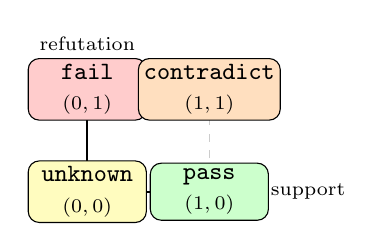
\begin{tikzpicture}[font=\small, x=1.55cm, y=1.30cm]
  \draw[->, thick] (-0.22,0) -- (1.42,0) node[right, font=\scriptsize] {support};
  \draw[->, thick] (0,-0.22) -- (0,1.28) node[above, font=\scriptsize] {refutation};
  \draw[gray!40, dashed] (1,0) -- (1,1) -- (0,1);
  \node[draw, rounded corners, fill=yellow!25, align=center, inner sep=2pt, minimum width=1.5cm]
    at (0,0) {\texttt{unknown}\\\scriptsize$(0,0)$};
  \node[draw, rounded corners, fill=green!20, align=center, inner sep=2pt, minimum width=1.5cm]
    at (1,0) {\texttt{pass}\\\scriptsize$(1,0)$};
  \node[draw, rounded corners, fill=red!20, align=center, inner sep=2pt, minimum width=1.5cm]
    at (0,1) {\texttt{fail}\\\scriptsize$(0,1)$};
  \node[draw, rounded corners, fill=orange!25, align=center, inner sep=2pt, minimum width=1.5cm]
    at (1,1) {\texttt{contradict}\\\scriptsize$(1,1)$};
\end{tikzpicture}
\caption{Four-state verdicts as Belnap states over \emph{registered evidence}.
\texttt{unknown} means ``not registered either way'', never ``no detector exists''; asset
availability is separate per-item metadata.}
\label{fig:belnap}
\end{figure}

\paragraph{Apparatus mechanisms (summary; details in Appendix~\ref{app:formal}).}
\texttt{artifact}$\to$\texttt{verifier}$\to$\texttt{verdict}$\to$\texttt{ledger}: knowledge
cards with a forced \emph{provenance/semantic-scope} split (\S\ref{sec:prov}); rule-based
verdicts; content-addressed evidence; a kernel-independent meta-state reconciler
(\S\ref{sec:reconciler}); and an append-only ledger under a zero-change red line.

\paragraph{Provenance vs.\ semantic scope.}
\label{sec:prov}
Provenance completeness and semantic-scope completeness are recorded separately, because a
provenance-complete assertion can still be misused outside its scope; the mechanism is in
place, the semantic-scope backfill is empty, and that directly limits external validity.

\paragraph{Meta-state reconciler.}
\label{sec:reconciler}
A kernel-independent script rescans ground-truth sources against the baseline and exits
non-zero on mismatch; assertions may hard-code a \emph{caliber}, never a
\emph{measurement}. Residual: ``kernel-independent'' means it does not import the kernel,
not that a third party wrote it.

\paragraph{Integrity mechanism.}
Evidence is content-addressed and the current state is protected by hash-chained roots over
controlled directories. This is \textbf{tamper-evident current-state integrity with partial
historical reproducibility}---\emph{not} an immutable log: an actor controlling both the
artifacts and the root can recompute both; ledger events do not yet carry a ruleset hash, so
historical states are reproducible only under an unchanged-ruleset assumption
(Appendix~\ref{app:pinning}).

% =====================================================================
\section{The Evaluator-Audit Protocol}
\label{sec:method}
% =====================================================================
We state the protocol abstractly; it is executable on our apparatus and transferable to
other measurement devices (any setting with samples, instruments, and a claimed rate).

\subsection{Claim declaration}
Every quantitative claim must declare its caliber $Q=(D,A,E,\Theta,P)$:
$D$ = dataset (samples and their provenance), $A$ = asset/instrument set, $E$ = environment
set (one or more profiles), $\Theta$ = configuration set (flags, levels, timeouts),
$P$ = protocol (pre-registration, seeds, statistical rules). A claim without $Q$ is not
falsifiable and is excluded from the paper's findings. Example: Finding~1's
$Q_1$ = (A5 held-out split, $n{=}566$; eight assets; WSL g++~13.3 profile; $k{=}4$;
frozen pre-registration with 2000 budget draws).

\subsection{Eight failure modes}
For each mode we give the definition, the identification signal used in our audit, and the
concrete instance found (all instances are documented in the appendices).

\begin{enumerate}\itemsep2pt
\item \textbf{Caliber drift.} The same evidence is scored under a changed caliber
(denominator, flags, or counting rule), so the reported rate moves without any capability
change. \emph{Signal:} re-binning identical raw counts under alternative denominators.
\emph{Instance:} unknown$\to$miss re-binning moves corpus recall by $+9.9$pp with the
\emph{same} 40 catches; a flag change once moved holdout recall $66.7\%\to87.5\%$ with the
detector untouched (Appendix~\ref{app:tables}, \ref{app:incidents}).
\item \textbf{Degenerate components.} Assets that cannot inform about the sampled defects are
still funded, so part of a ``selection gain'' is avoidance of zero-information slots, and
part of a pooled rate is a composition effect. \emph{Signal:} remove degenerate assets;
re-run selection at the same budget. \emph{Instance:} Finding~1 ($+24.0$pp collapses).
\item \textbf{Label corruption.} The measured object moves rather than the instrument: a
reported subset of ``20 samples'' contained 7 true errors; three sampled labels contradict
their own code in a later audit. \emph{Signal:} independent re-labeling; cross-source
consistency scans.  \emph{Instance:} \S\ref{sec:exp} Finding~4, \S\ref{sec:validity} T1.
\item \textbf{Environment loss.} The declared environment is part of the instrument; if it is
absent, capabilities disappear. \emph{Signal:} re-measure under the reduced profile with
three-component accounting (catch rate, unknown rate, conditional recall)---reporting a single
recall hides the loss. \emph{Instance:} Finding~3 ($59.09\%\to23.64\%$, unknown unchanged).
\item \textbf{Denominator changes.} Rates computed on different base populations are compared
as if comparable; unknown handling is the canonical case. \emph{Signal:} recompute every
rate under all defensible denominators and publish the spread. \emph{Instance:} the
$+9.9$pp caliber effect above; 38.4\% vs 61.6\% readings of the same matrix.
\item \textbf{Source/template dependence.} Samples share templates, so effective sample size
is far below nominal. \emph{Signal:} template-family-aware re-splitting and cluster
bootstrap. \emph{Instance:} design effect $\approx4.1$--$4.3$ (effective
$n\approx133$--$140$), CI widening $1.78$--$2.10\times$ (Appendix~\ref{app:a5full}).
\item \textbf{Comparator unfairness.} Cross-tool comparisons silently change environment,
timeout, calibration selection, or the use of post-hoc defensive calibers.
\emph{Signal:} predeclare configurations; report primary caliber even when it fails.
\emph{Instance:} our own E9 (Appendix~\ref{app:clangtidy}).
\item \textbf{Capability-boundary blindness.} Aggregate rates are silent about what the
instrument cannot see. \emph{Signal:} per-family blind-spot maps; per-asset contribution
under leave-one-out. \emph{Instance:} Finding~2 ($38.4\%$; $13$ of $34$ types $>50\%$ blind).
\end{enumerate}

\subsection{Falsification procedure}
For every headline claim: (i) state the claim; (ii) expose its hidden assumption;
(iii) construct the adversarial control that targets that assumption; (iv) re-measure on the
same held-out samples under the same caliber; (v) apply a predeclared decision rule.
We walk one claim end-to-end:

\emph{Claim.} ``Failure-driven asset selection improves recall over budget-matched random
selection.'' \emph{Hidden assumption.} All eight assets can inform about the sampled defects,
so selection quality (ranking) is what moves the rate. \emph{Adversarial control.} Remove the
three degenerate assets and re-run the same algorithm against the same random control at the
same budget; additionally clone-family re-split and cluster bootstrap. \emph{Re-measurement.}
Full pool: $+24.0$pp (CI $[+20.5,+27.5]$, $p{=}2.3\times10^{-41}$, $n{=}566$). Degenerate-free
pool: at $k{=}4$ random draws the same four assets ($\Delta{=}0.0$, $p{=}1.0$); at
$k\le3$, $+7.4$--$+11.3$pp survives, with effective $n\approx133$--$140$.
\emph{Decision rule.} A claim ``survives'' only if the effect remains non-zero and significant
under the degenerate-free control; otherwise it is graded \emph{collapses} (as a mechanism
claim) while the composition finding is registered as the real result. \emph{Outcome:}
collapses as stated; the audited version (Finding~1) survives.

\subsection{Four audit outcomes}
Each audited claim receives exactly one of:
\textbf{survives} (effect retains sign and significance under all predeclared adversarial
controls), \textbf{weakened} (retains sign, loses magnitude or significance under at least
one control), \textbf{collapses} (sign or significance lost under a control that directly
targets the hidden assumption), \textbf{unresolved} (controls cannot be run under the current
declared environment/caliber---the honest state for e.g.\ cross-regime comparisons). Findings
\S\ref{sec:exp} carry these grades; \S\ref{sec:validity} records what stays unresolved.

% =====================================================================
\section{Experimental Design}
\label{sec:protocol}
% =====================================================================
\paragraph{Datasets (never merged).}
\emph{Synthetic corpus} (1147 samples): self-authored C++ assertions with planted defects
across 34 normalized types (8 families), including 64 corpus-null controls and 35 hung
samples. \emph{Source-derived real-defect corpus} (110 samples): minimal reconstructions of
defects from 30+ real projects (CVE/NVD-verified mechanisms, responses frozen; \emph{not}
original project code---reconstruction loses build-system and cross-module fidelity). We
therefore name it \textbf{source-derived reconstruction}, never ``naturalistic'' evidence;
provenance is recorded as a three-value schema (self-authored /
source-derived-reconstruction / original-external-artifact). A 10-sample counting-caliber
difference between the A5 matrix ($n{=}1137$, after de-duplication) and the blind-spot map
($n{=}1147$, pre-de-duplication superset) is documented as two counting calibers of one
population, not a contradiction.

\paragraph{Blind holdout discipline.}
Primary rates come from a held-out split with failure-hit derivations disjoint from
evaluation; A5 evaluation runs on $n{=}566\gg138$; headline holdout/corpus rates
($n{=}41/64$) are reported with the caveat that the random arm at that denominator is an
instrument-level proxy, so only \emph{direction} is claimed (Appendix~\ref{app:tables}).

\paragraph{Baselines.}
Three arms, all budget-matched: \textbf{FD} (failure-driven selection), a
\textbf{static calibration arm} (the static gate re-binned under the same denominator---a
caliber reference, \emph{not} an independent verifier), and \textbf{random} (the control
separating ``failure-driven'' from ``spends more budget''). Ablations A0--A5 are
design-registered; \textbf{A5 has run} ($n{=}566$); A0--A4 remain unrun and are marked as
such wherever referenced.

\paragraph{Environments.}
Four profiles are declared: \texttt{wsl-gcc-13.3} (asan/ubsan/tsan, primary),
\texttt{windows-native-mingw} (compiler-warn/cross-compile/linker; sanitizers unavailable),
\texttt{wsl-clang-18.1.3} (200-sample stratified replication), and MSVC/clang-cl (absent on
this machine, declared unavailable---not simulated). Profile membership is printed with
every run; cross-profile numbers are never subtracted silently
(\S\ref{sec:exp}~Finding~3, Appendix~\ref{app:reframe689}).

\paragraph{Statistical caliber (frozen).}
Seed for every stochastic step; cluster-aware reporting (design effect $\approx4.2$);
exact McNemar for paired contrasts with Clopper--Pearson intervals; Holm/Bonferroni over
pre-registered contrasts; TOST for equivalence claims (added in 689);
$k$-sweeps and exploratory denominators reported as exploratory. \label{sec:baseline}
Post-hoc power is never presented as design power.

\paragraph{Pre-specified audit decisions.}
Before re-measurement we fixed: (a) degenerate-asset removal is the primary control for
selection claims; (b) environment-aware accounting requires three components, and a missing
profile caps the outcome at ``unresolved''; (c) equivalence requires TOST, never a
non-significant difference test; (d) the evolution hypothesis is falsified if the executable
operator cannot beat frequency-based selection at any predeclared tier.

% =====================================================================
\section{Findings: What Survives an Audit?}
\label{sec:exp}
\label{sec:analysis}
% =====================================================================
All numbers are recomputed from artifacts (Appendices~\ref{app:a5full},
\ref{app:reframe689}); intervals are Clopper--Pearson 95\% unless stated. Each finding
states the audited claim, the control, and the outcome grade.

\paragraph{F1. A $+24$pp ``selection gain'' is mostly measurement-pool composition
(\textbf{collapses as stated; composition finding survives}).}
A5's budget-matched control reports FD $54.6\%$ vs.\ random $30.6\%$
($\Delta{=}+24.0$pp full pool) on $n{=}566$. The adversarial control (remove three degenerate
assets; same algorithm, same budget) collapses the $k{=}4$ contrast to $0.0$pp
($p{=}1.0$): random's draw is then the same four assets. The composition contribution is
$+24.03$pp at the single $k{=}4$ caliber and $\approx+12.8$pp at the mean caliber; the
mechanism-level effect survives at $+7.4$--$11.3$pp ($k\le3$) with effective
$n\approx133$--$140$ after clone-aware re-splitting (design effect $\approx4.2$; CI widening
$1.78$--$2.10\times$). \emph{Reading:} a seemingly very large evaluator improvement was
substantially an artifact of measurement-pool composition. \emph{Cross-check:} the same
collapse reproduces on the source-derived corpus: at $k{=}1..7$ the executable operator's
literal selections coincide with greedy in every tier ($\Delta{=}0.0$pp).

\paragraph{F2. The instrument has a structured capability boundary (\textbf{survives}).}
Blind-spot ratio \textbf{38.4\%} ($440/1147$)---an \emph{instrument-boundary} statistic for
this corpus and this eight-asset instrument, expected to move when either changes.
\textbf{13 of 34} normalized types exceed $50\%$ blindness. Blindness is organized by defect
\emph{semantics}, not severity: family-level blindness spans memory $\approx15.7\%$ to
link/ODR $\approx67.7\%$, while CRITICAL/HIGH/MEDIUM real defects all detect at $60$--$62\%$;
parsing/multimedia real defects detect at $86.96\%$, OS/kernel at $30.77\%$, web-server
logic at $0\%$. On the real corpus, \textbf{41.5\%} of catches are solo-asset; asan alone
holds 18; removing asan drops detection $59.09\%\to42.73\%$. Semantic/logic families are
harder on real defects than on synthetic ones (type punning $-52.2$pp, logic $-22.5$pp,
data race $-20.7$pp; type-level, all reported in Appendix~\ref{app:reframe689}). This is a
major finding, not a limitation.

\paragraph{F3. Environment silently changes conclusions (\textbf{survives}).}
Under the declared WSL profile, the real corpus detects at 59.09\% ($65/110$); under the
reduced native profile (compiler-warn/cross-compile/linker only) it drops to
\textbf{23.64\%} ($-35.45$pp) with \emph{no} unknown increase: 39 catches depend on Linux
sanitizers, and the un-aware protocol records the missing measurements as misses, so guards
stay green while the conclusion silently changes. Same-OS compiler substitution (g++$\leftrightarrow$clang
on 200 paired samples) is benign: 93.5\% agreement, $\kappa{=}0.864/0.843$, $\Delta$catch
$\le2$pp, $\Delta$unknown $\le1.5$pp. Three-component accounting
(catch rate / unknown rate / conditional recall) is the minimum caliber that exposes the
difference; the native profile's sanitizer absence is an \emph{architectural inference}
(clang-cl/MSVC not present), declared as such. \emph{Reading:} environment is part of the
measurement, not a reproducibility footnote.

\paragraph{F4. ``Similar rates'' hide a composition offset; equivalence is not
established (\textbf{weakened}).}
The real 59.09\% vs.\ synthetic 61.64\% comparison previously carried a ``$p{=}0.60$'' that
must not be read as equivalence. A two-one-sided-test audit at $\pm10$pp \textbf{does not
pass}: 90\% CI $[-10.61,+5.52]$pp, $p_{\mathrm{TOST}}{=}0.064$; the minimum passing margin is
$10.61$pp ($11.67$pp under a conservative design-effect adjustment). \emph{Standardization}
answers why the headline rates look similar: re-weighting the synthetic family rates by the
real family composition raises the synthetic prediction to $77.01\%$---a
\textbf{$-17.92$pp} forward difference---while the reverse weighting nearly closes
($+1.70$pp); i.e.\ the overall similarity is produced by opposed composition effects
(real defects concentrate in strong families: bounds+memory+integer $=64.5\%$ of samples),
not by equal capability. Type-level standardization is directionally identical
($-13.52$pp). \emph{Naming correction:} source-derived reconstruction $\neq$ naturalistic
artifact; a three-value provenance schema is adopted.

\paragraph{F5. The evolution hypothesis fails (\textbf{the audited claim collapses; the
negative result is the finding}).}
Failure-driven evolution was the original thesis. Audited: the executable operator
$E$ (scored selection over failure/novelty/cost/redundancy) is \textbf{selection-identical}
to frequency-only and set-cover greedy in \textbf{14/14} pool$\times k$ blocks (in literal
mode, novelty is mathematically equivalent to failure; the uniqueness variant changes
selection in 11/14 blocks but adds no recall); on the real corpus, $k{=}1..7$ deltas are all
$0.0$pp; the best of 3/14 improving tiers is $+1.41$pp, $p{=}0.302$. \emph{Analysis, not
apology:} asset selection here is monotone submodular with a small asset universe, where
simple optimal selection already exists (all 17496 triples checked; greedy attains ratio
$1.0$; adaptive ceiling only $+2.29$pp)---\textbf{the apparent need for sophisticated
evaluator evolution can disappear once the evaluator-selection problem is correctly
formalized}. We also disclose that FD currently lacks a mechanism that exceeds a naive
frequency baseline. What the evolution loop retains is governance value: it forces failures
to become explicit, registered, and re-measured---falsifiability, not recall.

% =====================================================================
\section{Synthesis: Five Rules for Auditable Evaluators}
\label{sec:synthesis}
% =====================================================================
From the five audits we distill five reusable rules (each instantiated in Queyi and stated
so they transfer beyond C++ verification, e.g.\ to LLM evaluation and benchmark governance):
\begin{enumerate}\itemsep2pt
\item \textbf{R1 --- Every claim carries its caliber.} Publish $(D,A,E,\Theta,P)$ with the
number; a rate without a caliber is not an observation (\S\ref{sec:threat}, Eq.~\ref{eq:tuple}).
\item \textbf{R2 --- Unknown is not miss.} Report unknowns separately and never let a missing
measurement enter a denominator as a failure (Finding~3).
\item \textbf{R3 --- Capability boundaries accompany headline rates.} Every aggregate rate
travels with its blind-spot map and per-asset dependence (Finding~2).
\item \textbf{R4 --- Environmental validity is part of the measurement.} Declare environment
profiles, print available-asset manifests, and cap conclusions at ``unresolved'' when the
declared profile cannot be satisfied (Finding~3).
\item \textbf{R5 --- Apparent improvement must survive composition and matched-control
audits.} Remove degenerate components, re-run at matched budget, and re-split by template
family before calling a delta an improvement (Finding~1, F5).
\end{enumerate}
The AGEA abstraction (assets--governance--evolution--accountability) and the submodular
selection formalization are kept as \emph{tools} supporting R5, not as contributions
(Appendices~\ref{app:formal}, \ref{app:submodular687}).

% =====================================================================
\section{Threats to Validity}
\label{sec:validity}
% =====================================================================
We report five threat classes with direction and mitigation status (the 19-item table and
quantified residuals are in Appendices~\ref{app:tables}, \ref{app:threats_quantified}).

\paragraph{T1 --- Label validity (\emph{unresolved}).}
All rates rest on single-annotator labels; there is \textbf{no human inter-annotator
agreement}. The $\kappa$ values in this paper ($0.77$, $n{=}131$; $0.73$, $n{=}287$) are
\textbf{AI self-consistency, not human IAA}, and must not be cited as validation. A
two-annotator blind protocol with a de-identified 145-sample package, 10 calibration items,
and pre-registered thresholds (verdict $\kappa\ge0.8$; family $\kappa\ge0.7$) is
\emph{designed and packaged but not executed} (Appendix~\ref{app:reframe689}); until then,
label-sensitive conclusions are flagged (labels can move the absolute blind-spot rate
$6.6\%\to14.3\%$ under $\le15\%$ flips, though contrast directions are stable).

\paragraph{T2 --- External validity (\emph{partially mitigated}).}
One language (C++), one apparatus of eight assets, and a synthetic corpus whose defects were
designed to be observable (a selection bias we now quantify rather than hide: Finding~4).
The 110-sample source-derived corpus improves ecological validity but is
\emph{reconstruction}, not production code; type coverage reaches 9 of the 10 targeted
families.
\label{sec:claim}
Claim boundary: a \texttt{catch} is evidence within a boundary, never semantic truth; the
e-process remains exploratory and supports no confirmatory claim
(Appendix~\ref{app:eprocess}).

\paragraph{T3 --- Environment validity (\emph{partially mitigated}).}
The primary profile is WSL-bound; without it, the measured capability drops 35.45pp
(Finding~3). The native profile's sanitizer absence is an architectural inference (no
clang-cl/MSVC on the machine); containerized reproduction and a native three-asset re-run
are specified with decision criteria but not executed (Appendix~\ref{app:reframe689}).
Toolchain asymmetry (static tools on MinGW vs.\ dynamic assets on WSL) makes some
comparisons observational only.

\paragraph{T4 --- Dependence and clustering (\emph{mitigated}).}
Synthetic samples share templates; clone-family-aware re-splits and a family-level cluster
bootstrap give effective $n\approx133$--$140$ (design effect $\approx4.1$--$4.3$; CIs
widened $1.78$--$2.10\times$). All headline contrasts are reported under both calibers.
Single-run grid instability ($\approx5\%$ of cells flip) bounds point estimates by roughly
$\pm2$pp and is not folded into the intervals.

\paragraph{T5 --- Instrument scope and stability (\emph{mitigated}).}
Eight assets; two are declared-unavailable (never funded); detection rides
disproportionately on asan (18 solo catches); a removed-asan control changes the real-corpus
rate by $-16.36$pp. Cross-run stability: 5\% grid flips; the shadow-mapped
toolchain replication agrees at 93.5\%.

% =====================================================================
\section{Conclusion}
\label{sec:conclusion}
% =====================================================================
We found that evaluator claims that initially appear robust can materially weaken or
collapse when the evaluator itself is audited, and we provide an executable protocol for
detecting that collapse. On a software-verification apparatus: a $+24$pp selection gain was
mostly measurement-pool composition; the instrument is blind to 38.4\% of its corpus in a
family-structured way; losing the declared environment silently cut real-defect detection by
35pp with no warning; synthetic-vs-real similarity failed a TOST equivalence test and is
explained by a $-17.9$pp composition offset; and failure-driven evolution produced no
measurable recall advantage over frequency selection---the audited claim collapsed, and we
report the collapse as the result. What remains is a protocol, five rules, and a measured
map of what survives.

\paragraph{Future work.}
Execute the human annotation (the single most important pending item); reproduce a small set
of original-project builds to test reconstruction fidelity; add an LLM-as-verifier arm and
semantic/logic-layer verifiers; extend the audit protocol across languages/domains; and
invite third-party replication challenges under the published caliber.

\clearpage
\label{page:endmain}% records the page where the main text ends (for the 9-page check)
\bibliographystyle{plainnat}
\bibliography{queyi_refs}

\newpage
\appendix

\section{LLM Arm and External Anchor (details)}
\label{app:extra}
\paragraph{E7 --- LLM judge arm (result \emph{opposite} to expectation, registered as such).}
\textbf{GLM-4} (temperature 0.01, prompt v1) caught \textbf{12/12} errors vs.\ FD's 6/12 on the same
subset but produced \textbf{4/8 false positives} (50\%) on controls (exact McNemar favours the LLM,
$b{=}0$, $c{=}6$, $p{=}0.031$). \textbf{All four pre-registered hypotheses failed}: more sensitive,
far less specific. Caveats: some samples carry \texttt{answer\_leak\_risk} (fixture comments may hint
the answer); single model, single prompt. This is the empirical case for T15---an LLM may
\emph{propose}, but its output never becomes a verdict.

\paragraph{E8 --- External anchor (C++ Core Guidelines; H2 misses by 0.8pp).}
We scanned the official \textbf{C++ Core Guidelines} (\texttt{isocpp/CppCoreGuidelines}, sha256
\texttt{27b53e7d\ldots}), one compilable snippet per rule (87 rules). Reported separately because
targets differ: \textbf{A} verbatim guideline snippets (35 measurable, \textbf{28.6\%}) and \textbf{B}
reconstructed UB fragments (15, \textbf{80.0\%}); total \textbf{44.0\%} over 50. A is low because
most guideline text is stylistic advice---``no detection'' there is \emph{expected}; B is our own
reconstruction (\texttt{verified\_source=false}), an \emph{upper bound}. Pre-registered: H1/H3 hold,
\textbf{H2 misses by 0.8pp} and is registered as \emph{not} passed (harness \texttt{prelude\_v1}
added post-registration because raw compilability was 11/60; logged).

\section{Threat, Validity and Evolution Tables}
\label{app:tables}
Layer read at 672h (k/n per layer; layers are never merged): corpus sanitizer
\textbf{85.3\%} (29/34), compiler-warn \textbf{50.0\%} (9/18), cross-compile \textbf{16.7\%}
(2/12)---three further layers lack local detectors and therefore claim \emph{no} rate; holdout
sanitizer \textbf{84.6\%} (33/39). These denominators are recomputed from the landed reveal
artifacts and are the source of the abstract's layered read.

\begin{table}[t]
\caption{E4. Ablation groups A0--A5. Each row writes its hypothesis \emph{before} results; A0--A4 remain design-registered and \emph{unrun} (declared as such in the main text); only A5 has run.}
\label{tab:e4}
\centering
\footnotesize
\begin{tabular}{@{}clp{2.9cm}p{3.1cm}p{4.7cm}@{}}
\toprule
ID & Remove/change & Hypothesis & Primary metric & Result \\
\midrule
A0 & Full system (baseline) & --- & detection rate & \textit{not run} \\
A1 & $-$failure-derived rules (post-657 ruleset) & H: detection drops & $\Delta$ detection vs.\ A0 & \textit{not run} \\
A2 & $-$holdout isolation (blind$\to$dev) & H: overfitting (dev$\uparrow$, blind flat) & dev vs.\ blind recall & \textit{not run} \\
A3 & $-$provenance (boundary-triple check) & H: false-pass rate rises & false-pass rate & \textit{not run} \\
A4 & $-$mutation (L1 self-justification) & H: internal strength drops & mutation kill (internal) & \textit{not run} \\
A5 & random-budget control & H: below A0 & $\Delta$ detection vs.\ A0 & \textbf{run at full scale (676f)}: $n{=}566$ eval; vs Random \textbf{+24.0}pp [+20.5, +27.5] ($p{=}2.3{\times}10^{-41}$), vs Static \textbf{+29.9}pp ($p{=}1.9{\times}10^{-31}$); Static contrast survives the parallel analysis (\textbf{+30.6}pp), Random contrast collapses to \textbf{0.0}pp $\Rightarrow$ \texttt{uninterpretable} \\
\bottomrule
\end{tabular}
\end{table}
\begin{table}[h]
\caption{E5. Paired contrasts on the same samples. $b$ = FD catch \& opponent miss;
$c$ = opponent catch \& FD miss. All four contrasts have $c=0$ (the opponent's catches are a
subset of FD's), so the difference comes entirely from samples only FD catches.}
\label{tab:e5}
\centering
\footnotesize
\begin{tabular}{@{}llrll@{}}
\toprule
Contrast & Set & $(b, c)$ & exact McNemar $p$ & Cohen's $h$ \\
\midrule
FD vs.\ Static & holdout ($n{=}41$) & (33, 0) & $2.3\times10^{-10}$ & \textbf{1.98} (large) \\
FD vs.\ Static & corpus ($n{=}64$) & (29, 0) & $3.7\times10^{-9}$ & \textbf{0.97} (large) \\
FD vs.\ Random$\dagger$ & holdout ($n{=}41$) & (30, 0) & $1.9\times10^{-9}$ & \textbf{1.65} (large) \\
FD vs.\ Random$\dagger$ & corpus ($n{=}64$) & (26, 0) & $3.0\times10^{-8}$ & \textbf{0.85} (large) \\
\bottomrule
\end{tabular}
\end{table}

\begin{table}[h]
\caption{Baselines and their alignment conditions (moved from main text; referenced in \S\ref{sec:baseline}).}
\label{tab:baseline}
\centering
\footnotesize
\begin{tabular}{@{}lp{5.2cm}p{6.4cm}@{}}
\toprule
Baseline & Definition & Alignment \\
\midrule
B1 static gate & static rules only (no runtime evidence) & same corpus, same verdict granularity \\
B2 static $+$ mutation & static rules $+$ mutation testing & same as above $+$ same mutation budget \\
\textbf{B3 budget-matched random} & random evidence acquisition under \emph{equal budget} & same budget (time/calls), same corpus, same flags \\
\bottomrule
\end{tabular}
\end{table}

\begin{table}[h]
\caption{Four-state verdict (moved from main text; referenced in \S\ref{sec:method}).}
\label{tab:verdict}
\centering
\footnotesize
\begin{tabular}{@{}lll@{}}
\toprule
State & Meaning & Action \\
\midrule
\texttt{pass} & evidence supports the assertion; boundary triple complete & may enter the teaching ledger \\
\texttt{fail} & evidence contradicts the assertion & counterexample to the teaching set \\
\texttt{unknown} & insufficient evidence or detector unavailable & never recorded as pass/miss; reported separately \\
\texttt{contradict} & two pieces of evidence conflict (e.g.\ cross-compiler) & escalated to human review; no machine pick \\
\bottomrule
\end{tabular}
\end{table}

\begin{table}[h]
\caption{E2. Caliber ablation (same raw counts, different denominator). The 669d table
(87.5/82.4/82.4 and 43.8/37.8/35.0) is \emph{retired}: its denominators are the pre-expansion
16/17/40. Moved from main text; referenced in \S\ref{sec:exp}.}
\label{tab:e2}
\centering
\footnotesize
\begin{tabular}{@{}lp{3.6cm}p{3.6cm}p{3.6cm}@{}}
\toprule
Arm & Caliber & holdout (CP 95\%) & external (CP 95\%) \\
\midrule
\textbf{A (main; drop unknown)} & denominator $=$ catch$+$miss & \textbf{82.9\% (34/41) [67.9, 92.8]} & \textbf{62.5\% (40/64) [49.5, 74.3]} \\
B (unknown $\to$ miss) & denominator incl.\ detector-unknown & 81.0\% (34/42) [65.9, 91.4] & 54.8\% (40/73) [42.7, 66.5] \\
C (unknown $+$ not\_error) & denominator $=$ all samples & 81.0\% (34/42) [65.9, 91.4] & 52.6\% (40/76) [40.8, 64.2] \\
\midrule
$\Delta$(A$-$C) & & $+1.9$pp & $\mathbf{+9.9}$pp \\
\bottomrule
\end{tabular}
\end{table}

\begin{table}[h]
\caption{E1. Three arms on the same samples. Static is a caliber re-binning; Random$\dagger$ is a
proxy (the real B3 needs the split-repo \texttt{select\_assets}). Moved from main text; referenced in \S\ref{sec:exp}.}
\label{tab:e1}
\centering
\footnotesize
\begin{tabular}{@{}lp{2.7cm}p{2.4cm}p{1.7cm}p{1.5cm}@{}}
\toprule
System & Blind holdout (CP 95\%) & Corpus meas.\ (CP 95\%) & Defect & Control FPR \\
\midrule
Static (caliber re-bin) & 2.4\% (1/41) [0.1, 12.9] & 17.2\% (11/64) [8.9, 28.7] & 100\% (6/6) & --- \\
Random$\dagger$ (proxy) & 9.8\% (4/41) [2.7, 23.1] & 21.9\% (14/64) [12.5, 34.0] & N/A & --- \\
\textbf{FD (failure-driven)} & \textbf{82.9\% (34/41) [67.9, 92.8]} & \textbf{62.5\% (40/64) [49.5, 74.3]} & 100\% (6/6) & 0.0\% (0/11) [0.0, 28.5] \\
$\Delta$(static$\to$FD) & \textbf{+80.5pp} [68.4, 92.6] & \textbf{+45.3pp} [33.1, 57.5] & 0 & --- \\
$\Delta$(random$\dagger\to$FD) & \textbf{+73.2pp} [59.6, 86.7] & \textbf{+40.6pp} [28.6, 52.7] & N/A & --- \\
\bottomrule
\end{tabular}
\end{table}

\section{Rule Pinning and e-Process (details)}
\label{app:pinning}
\textbf{Rule-version pinning (design principle; manifest-level today).} Rules inevitably evolve, so
a ledger that records only verdicts cannot let a third party recompute a one-year-old decision: the
ruleset of the day must be pinned. We snapshot the ruleset and hash the canonicalised manifest into
\texttt{rules\_manifest\_sha256}, archived append-only, with each ledger event double-referencing
that hash and the evidence-toolchain snapshot. \textbf{Current state (measured):} the manifest
exists (\texttt{rules\_sha256}, version 1.0.0, 67 rules), but the \textbf{452 ledger events do not
yet carry the field}---backfilling is registered as future work, so today a historical recomputation
must \emph{assume} the ruleset was unchanged.

\textbf{e-process (moved).} The sequential-testing layer is described in full in
Appendix~\ref{app:eprocess}; it is \textbf{exploratory} and supports no confirmatory claim in this
paper.

\subsection{E-Process (exploratory)}
\label{app:eprocess}
\textbf{EXPLORATORY --- not pre-registered, not used for confirmatory claims.} $\mu_0$, the
alternative grid and the mixing prior are unfrozen, the implementation is not in CI, and no claim
depends on an e-value. \textbf{Why at all.} The ledger accumulates items one at a time, yet rates are
reported at snapshots---\emph{peeking}. Treating each event as a binary observation and mixing
likelihood ratios gives an \emph{e-process} (a supermartingale with expectation 1 under $H_0$):
cumulative e-values multiply across batches; reject when $\sup_t e_t\ge1/\alpha$ ($20$ at
$\alpha{=}0.05$); Ville's inequality keeps peeking anytime-valid. Measured FD contrasts reach
e-values $\ge10^6$---\emph{exploratory} numbers only (a different $\mu_0$ gives different e-values,
so the margin is not evidence strength). \textbf{Honest boundaries:} the anytime-valid price is
threshold $\approx20$ vs.\ $\approx3.14$ fixed-sample ($\approx6.4\times$ in LR terms)---a safety
belt for expansion, not the primary test. \textbf{Difference from
CELEUS}~\cite{zhou2026celeus}: CELEUS saves samples in LLM evaluation; we provide
third-party-recomputable decisions over a knowledge-assertion ledger. Not first.


\begin{table}[t]
\caption{Evaluator-audit neighbours (metadata verified online 2026-10-07). Queyi's differences are in the audited \emph{object} (a software-verification evidence-acquisition apparatus, including caliber, composition, environment, labels and denominators) and in its negative findings---we do not claim priority~\cite{huang2026deepfact,zhang2026whogrades,sengupta2026anytimevalid,beyer2026svcomp}.}
\label{tab:positioning}
\centering
\footnotesize
\begin{tabular}{@{}p{1.7cm}p{2.6cm}p{2.9cm}p{1.8cm}p{1.6cm}p{1.9cm}@{}}
\toprule
Work & Object audited/evolved & Audit mechanism & Unknown & Env.\ modeled & Domain \\
\midrule
\textbf{Queyi} & software-verification evidence-acquisition apparatus & claim caliber + 8 failure modes + adversarial re-measurement + 4 outcomes & four-state, first-class & yes (tuple + 3-component metrics) & C++ assertions, 8 assets \\
DeepFact~\cite{huang2026deepfact} & benchmark labels and rationales (AtS loop) & verifier submits evidence; auditor adjudicates; benchmark updated before scoring & not explicit & no & deep-research factuality \\
Who Grades~\cite{zhang2026whogrades} & evaluation metric function (typed detectors) & locked-set audit + anchor guards (ablation: collapse without guards) & not explicit & no & LLM agent skills \\
SEA~\cite{sengupta2026anytimevalid} & agent policy (adapter + harness) & versioned harness + anytime-valid certificates & certificate budget & harness fixed, not audited & general agents \\
SV-COMP~\cite{beyer2026svcomp} & verifiers (ranked yearly on fixed tasks) & witness validation by independent tools & timeout$\approx$unsolved & containers (normalized) & C/Java/SV-LIB verification \\
HELM / cards~\cite{liang2023helm} & documents, not instruments & documentation checklists & no & reported, not audited & general ML \\
\bottomrule
\end{tabular}
\end{table}
\begin{table}[t]
\caption{What the current evidence does and does not support.}
\label{tab:claim}
\centering
\small
\begin{tabular}{@{}p{1.3cm}p{5.4cm}p{7.0cm}@{}}
\toprule
 & Claim & Evidence \\
\midrule
\cmark\ supported & High recall on \emph{seen} error types & holdout \textbf{82.9\%} (34/41) [67.9, 92.8]; corpus measurable \textbf{62.5\%} (40/64) [49.5, 74.3] (post-672h) \\
\cmark\ supported & Gates catch \emph{known} defects (change a number, go red) & range self-check 5/5 red; gate \texttt{overall=PASS} \\
\cmark\ supported & Current-state integrity is tamper-evident (with a declared threat model) & hash-chained roots over controlled directories detect changes to the current state; 452-event ledger unchanged; partial historical reproducibility only under an unchanged ruleset \\
\cmark\ supported & Caliber declarable and recomputable & three-arm caliber ablation; every rate carries a denominator \\
\cmark\ supported & On the same samples FD beats the static calibration arm and random$\dagger$ proxy arms & exact McNemar $p\le3.0\times10^{-8}$; Cohen's $h\ge0.85$; $\Delta$ lower bound $\ge$28.6pp (\S\ref{sec:exp}) \\
\cmark\ supported & On the \emph{visible} region, FD beats a budget-matched static calibration arm at scale & A5: +29.9pp ($p{=}1.9\times10^{-31}$), +30.6pp in the parallel analysis ($n{=}566$); unchanged under clone-family splitting (677b); effective $n\approx133$--$140$ \\
\cmark\ supported & A detector's capability boundary can be mapped and published & 1147-sample $\times$ 8-asset matrix \emph{on our corpus with our 8-asset instrument}: blind-spot ratio 38.4\%; 13/34 normalized types $>50\%$ blind; union of 6 assets 61.6\% vs best single 35.6\% (\S\ref{app:blindspot}). \emph{Instrument-boundary statistic, not a property of C++ defect detection} \\
\midrule
$\times$ not supported & Generalization to \emph{unseen} error types & all samples same-source; scope backfill 0/26 \\
$\times$ not supported & Absolute ``detection rate $X$\%'' & $n{=}41/64$, CI half-width $\approx$12pp; $\pm$5pp needs $n{=}236/378$ \\
$\times$ not supported & Better than a \emph{real} static detector / true B3, or ``FD beats same-budget random'' & static arm is a caliber re-binning; random$\dagger$ is a proxy; real interfaces BLOCKED; \textbf{A5 at full scale ($n{=}566$) is significant vs Static and robust in the parallel analysis (+30.6pp)}; vs Random it is \textbf{+11.31pp at $k{=}1$ on the degenerate-free pool} ($p{=}6.0\times10^{-8}$; 677c) and 0.0pp at $k{=}4$ (set collision $1/\binom54$); clone-aware splits leave both unchanged (677b) and the family-level cluster bootstrap gives effective $n\approx133$--$140$ $\Rightarrow$ \emph{direction-only} on a smaller selection effect ($\approx$\,$+7$--$12$pp) \\
$\times$ not supported & ``$F_1{=}1.0$ is calibrated'' & criterion and truth are same-source $\Rightarrow$ upper bound \\
$\times$ not supported & Mutation score as detection rate & core 96.5\% $\neq$ defect-detection rate~\cite{just2014mutants} \\
$\times$ \textbf{collapsed} & ``failure-driven evolution improves recall'' & the executable operator selection is identical to frequency and set-cover greedy (14/14 pool$\times k$ blocks; real corpus $\Delta{=}0.0$pp at $k{=}1..7$; best improving tier $+1.41$pp, $p{=}0.302$) $\Rightarrow$ reported as Finding~5, not a contribution (Appendix~\ref{app:operator683}) \\
\midrule
\multicolumn{3}{@{}p{13.7cm}@{}}{\textbf{Environment-conditioned (silent degradation when the profile changes):} real-corpus detection depends on the declared WSL sanitizer profile; without it the rate drops $59.09\%\to23.64\%$ with \emph{no} unknown increase and no guard turning red (Finding~3; 689 caliber). The native profile's sanitizer absence is an architectural inference (no clang-cl/MSVC on the machine).} \\
\bottomrule
\end{tabular}
\end{table}

The three tables below are moved here to keep the main text within the 9-page limit; their labels are unchanged, so all cross-references still resolve.

\begin{table}[t]
\caption{Threats, mitigations and residual risks.}
\label{tab:threats}
\centering
\small
\begin{tabular}{@{}p{0.5cm}p{4.6cm}p{4.2cm}p{4.6cm}@{}}
\toprule
\# & Threat & Mitigation & Residual \\
\midrule
T1 & Self-justification (toolchain proves itself) & kernel-independent reconciler (\S\ref{sec:reconciler}) & reconciler still needs human review; \texttt{--check} $\neq$ independent implementation \\
T2 & Self-made distribution bias & blind holdout + external corpus (D2/D3) & small external sample \\
T3 & holdout leakage & irreversible reveal; holdout dir not scanned & 10 appended samples have no blinding \\
T4 & developer-knowledge bias & independent generation (A/B/C) & same-process context; not truly independent \\
T5 & caliber drift & meta-state reconciliation & covers registered fields only \\
T6 & semantic-scope misuse & forced provenance/scope split (\S\ref{sec:prov}) & scope completeness 0/26 \\
T7 & metric confusion (mutation $\to$ detection) & metric layering; mutation is self-justification only & external readers may still misread \\
T8 & selection bias (budget) & budget-matched random baseline (\S\ref{sec:baseline}); three arms \textbf{run} & random arm is an \emph{instrument-level proxy} (true B3 not rerun at 672h) \\
T9 & overfitting historical defects & blind D2 + external D3 & appended samples unblinded \\
T10 & reproducibility crisis & hash-chained roots + version capture + time anchor & OTS is a placeholder; WSL dependency undeclared \\
T11 & authority manipulation & 452-event ledger, zero-change red line & discipline, not cryptographic enforcement \\
T12 & unclear AI authorship & AI-use registry & contribution split remains a convention \\
T13 & \textbf{peeking / selective stopping}: the ledger accumulates while rates are reported at snapshots & frozen statistical plan; \textbf{e-process / confidence sequence} as a pre-committed expansion protocol (\S\ref{sec:method}) & nothing forces $\mu_0$ to be fixed in advance $\Rightarrow$ pre-registration required \\
T14 & \textbf{four-layer contamination}: literal / near-duplicate / semantic / procedural---can be ``inflated but reproducible'' & paired counterfactual probes (rename identifiers, change compiler/order); unsealing event log; four-layer de-duplication & passive cleaning is unreliable; probes need human reading \\
T15 & \textbf{untrusted LLM channel}: prompt injection / adversarial input (CVE-2025-59145 CamoLeak, CVSS 9.6; indirect-injection ASR 24--52.77\%) & prompt-level spotlighting/datamarking; structural schema check; \textbf{architectural: LLM output never becomes a verdict, ML detection warns but never blocks} & touch-point registry not done; the LLM arm's false-positive rate is 50\% (\S\ref{sec:exp}) \\
T16 & \textbf{small-sample poisoning}: \textbf{250} malicious samples (0.00016\% of tokens) reliably plant a backdoor---the decisive variable is the \emph{absolute count}; our $n{=}41/64$ lies in that range & canary cards; paired counterfactual probes; the reconciler uses a \emph{different} dependency set; candidates run sandboxed as untrusted code & no safety margin; passive cleaning unreliable (3\% poisoning moves the error rate 3\%$\to$24\%) \\
\bottomrule
\end{tabular}
\end{table}
\begin{table}[t]
\caption{Five validity layers: threat / mitigation / residual.}
\label{tab:validity}
\centering
\small
\begin{tabular}{@{}p{1.8cm}p{4.4cm}p{4.0cm}p{3.6cm}@{}}
\toprule
Layer & Threat & Mitigation & Residual \\
\midrule
Construct & \texttt{catch} $\neq$ truth; A/B/C split by detector availability not difficulty; mutation score not a detection proxy~\cite{just2014mutants}; \textbf{static arm is a caliber re-binning, not a re-run; random$\dagger$ is an instrument-level proxy, not B3} & caliber/denominator/opt\_levels/env stored with artifacts; dual-flag; three-state separation; proxy arms marked $\dagger$ and excluded from conclusions & cross-environment reproduction unverified (upgraded from ``residual'' to ``observed failure'': score drops without WSL); no independent label review; ``with/without runtime evidence'' vs.\ ``failure-driven'' not yet separated (needs ablation) \\
Internal & meta-Goodhart; budget selection bias; code changed without rerun & caliber three-step discipline; range self-check (5/5 turn red); budget-matched random control & guard does not rerun the detector, so the 666 incident can recur; A5 run but holds only as pool composition (\texttt{uninterpretable}); A0--A4 design frozen \\
External & small $n$ (holdout 21 / corpus 48 measurable); \textbf{expanded samples merged after reveal (no blind state: 10 holdout $+$ 20 corpus)}; same-source clustering; scope 0/26; single domain (C++) & layered reporting; two sample sets explicitly incomparable; unblinded samples explicitly flagged & static re-bin $+$ random$\dagger$ proxy \emph{run}; \textbf{real B3 BLOCKED}; only A5 run; reconciler is still our own; 0 third-party reproductions \\
Statistical & \textbf{small $n$ (41/64)} $\Rightarrow$ still-wide CIs; McNemar rests on the extreme $c{=}0$ structure; \textbf{control FPR 0.0\% (0/11)}; multiple comparisons; Wald invalid at small $n$; clustering; $p$ without effect size & frozen plan; CP primary, Wilson sensitivity; Fisher/Boschloo $+$ exact McNemar \emph{tool-implemented}; BH/Holm; difference $+$ CI $+$ effect size $+$ e-value required (the e-process is \emph{exploratory} and supports no confirmatory claim; Appendix~\ref{app:eprocess}) & $\pm$5pp needs $n{=}236/378$; $\pm$10pp needs $61/97$; $\Delta{=}15$pp needs $n\approx103$--173 (paired)---\textbf{A5 now has $n{=}566$ and clears this}, so power is no longer binding for A5, but the holdout/corpus headline ($n{=}41/64$) still has $\approx$12pp half-widths; magnitude not readable as exact; IRR not done \\
Temporal & OTS anchor expired~\cite{opentimestamps}; sample aging; environment drift (TSan intermittently fails under WSL high-entropy ASLR) & Merkle roots $+$ hash chain; versions captured with evidence & OTS not really anchored; re-pinning invalidates the anchor; WSL hard dependency undeclared \\
\bottomrule
\end{tabular}
\end{table}
\begin{table}[t]
\caption{E3. Cross-batch key metrics. \textbf{Un-pinned rows:} the 656 mutation cell (\,62.5\%, 30/48)
has \emph{no surviving artifact}---the current reports recompute to 110/114 and 130/159---and the 665
cell (66.7\%) comes from the retired single-flag (\texttt{-O1}) caliber, so neither may be read as a
reproducible result; they are kept only as a record of what was reported at the time.}
\label{tab:e3}
\centering
\small
\begin{tabular}{@{}llp{3.0cm}lp{3.0cm}@{}}
\toprule
Batch & New capability & holdout (true/caliber) & mutation core & Nature \\
\midrule
656 & core PBT/mutation & --- & \textbf{62.5\%} (30/48) & mutants out of range \\
660 & trace layer & true 7, \textbf{80.0\%} (small den.) & --- & label over-claim \\
665 & expand 20$\to$30 & true 17, \textbf{66.7\%} (single flag) & --- & denominator changed \\
666 & claimed dual & \textit{81.2\% never landed} & --- & code changed, no rerun \\
668 & dual-flag rerun & \textbf{87.5\%} (14/16) & --- & \textbf{caliber change} \\
669 & caliber ablation $+$ CI & 87.5\% [61.7, 98.4] & \textbf{96.5\%} (110/114) & mutation still internal \\
671a & expansion $+$ corpus dual-flag & \textbf{81.0\%} (17/21) [58.1, 94.6] (10 unblinded merged) & --- & \textbf{expanded re-estimate} \\
672h & re-expansion (21$\to$41 / 48$\to$64) & \textbf{82.9\%} (34/41) [67.9, 92.8] (20 unblinded merged) & --- & \textbf{expanded re-estimate (H4 corpus shift registered)} \\
\bottomrule
\end{tabular}
\end{table}

\section{Rule Manifest (67 rules)}
\label{app:rules}
The rule engine computes \texttt{len(RULES)}$=$\textbf{67}. By severity: \textbf{block 44 / warn 16
/ advice 7} (total 67). By kind: fact 61 / pedagogy 5 / meta 1. Fields:
\texttt{id, title, severity, kind, quadrant, scope, automated, basis, fix\_hint, check}.
\emph{Correction note:} an earlier draft wrote ``67 (block 0 / warn 176 / advice 55)''; recomputation
gives \textbf{44/16/7} (sum 67), and the old triple cannot be reproduced from the rule table. The
full 67-row list is generated by the command in Appendix~\ref{app:repro} and shipped with the
supplementary material.

\section{Formal Definitions and Gate Tiers (moved from main text)}
\label{app:formal}
This appendix holds the formal statement of \S\ref{sec:method} that was moved out of the main text
to stay within the page limit. Nothing here is new relative to v1.1.

\begin{figure}[t]
\centering
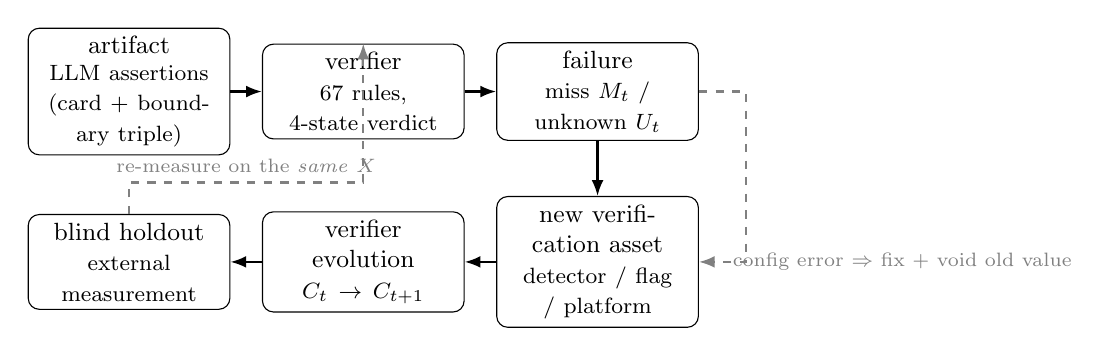
\begin{tikzpicture}[
  font=\small,
  box/.style={draw, rounded corners, align=center, inner sep=3pt, minimum height=9mm, text width=2.35cm},
  arr/.style={-{Latex[length=2mm]}, thick},
  fb/.style={-{Latex[length=2mm]}, dashed, thick, gray}
]
\node[box] (a) {artifact\\\footnotesize LLM assertions\\\footnotesize (card + boundary triple)};
\node[box, right=4mm of a] (b) {verifier\\\footnotesize 67 rules, 4-state verdict};
\node[box, right=4mm of b] (c) {failure\\\footnotesize miss $M_t$ / unknown $U_t$};
\node[box, below=7mm of c] (d) {new verification asset\\\footnotesize detector / flag / platform};
\node[box, left=4mm of d] (e) {verifier evolution\\\footnotesize $C_t \to C_{t+1}$};
\node[box, left=4mm of e] (f) {blind holdout\\\footnotesize external measurement};
\draw[arr] (a)--(b);
\draw[arr] (b)--(c);
\draw[arr] (c)--(d);
\draw[arr] (d)--(e);
\draw[arr] (e)--(f);
\draw[fb] (f.north) -- ++(0,4mm) -| node[pos=0.25, above, font=\scriptsize]{re-measure on the \emph{same} $X$} (b.north);
\draw[fb] (c.east) -- ++(6mm,0) |- node[pos=0.75, right, font=\scriptsize, align=left]{config error $\Rightarrow$ fix + void old value} (d.east);
\end{tikzpicture}
\caption{The failure-driven verification loop. Solid arrows form the main cycle; dashed arrows
are re-measurement and caliber correction. Tools: the rule engine (67 rules, four states), the
kernel-independent meta-state reconciler, and the counterfactual operator.}
\label{fig:loop}
\end{figure}

\paragraph{The audited apparatus.} The figure above is the object of the audit: an LLM emits assertions; a rule-based verifier yields four-state verdicts; registered failures (only legal input) drive capability changes; a blind holdout re-measures on the \emph{same} $X$; dashed arrows are re-measurement and caliber correction (a configuration error voids the old value).

\paragraph{Formal definitions (backing the three contributions).}
\emph{Verifier state} $\mathcal{C}_t$: the set of available evidence-acquisition means (detectors
$\times$ compilers $\times$ flags $\times$ platforms) at time $t$; its discrete form is the
67-rule set. \emph{Failure set} $F_t = \{x : v_t(x) \in \{\texttt{miss}, \texttt{unknown}\}\}$;
\texttt{miss} points directly at a capability gap, while \texttt{unknown} first needs attribution
(measurement-configuration error vs.\ capability gap). \emph{Evolution operator}
$\mathcal{C}_{t+1} = E(\mathcal{C}_t, F_t)$ with three checkable properties:
\emph{monotonicity} ($\mathrm{cov}(\mathcal{C}_{t+1}) \supseteq \mathrm{cov}(\mathcal{C}_t)$---
evolution never removes capability), \emph{minimality} (every application of $E$ must be triggered
by a \emph{registered} failure; no rule inflation without failure evidence), and
\emph{auditability} (each application leaves the triple (registered failure $f$, new rule $r$,
re-test record)). \emph{Information structure of the four states}: each verdict is a Belnap state
$(\mathrm{support},\mathrm{refutation})$ over registered evidence---\texttt{pass}$=(1,0)$,
\texttt{fail}$=(0,1)$, \texttt{unknown}$=(0,0)$, \texttt{contradict}$=(1,1)$---\emph{while
detector availability} is carried as \emph{separate metadata} per item, not as part of the Belnap
state. Merging \texttt{unknown} into \texttt{miss} or \texttt{pass} pollutes the denominator or
manufactures false confidence; the primary estimand therefore conditions on measurable samples
(denominator $=$ catch $+$ miss). \emph{Auditability conditions}:
origin traceability ($\forall v\, \exists (e,r): v = R_r(e)$), state reproducibility (a third party
rebuilds verdict-time inputs from on-disk artifacts), and tamper detectability (any change to a
controlled directory moves the Merkle root; the ledger is append-only)---jointly necessary, and
jointly met \emph{for the current state} only: ledger events do not yet carry a ruleset hash, so
historical replay assumes the ruleset was unchanged.

\paragraph{Evolution operator: executable form (677c).}
$E$ is instantiated as a one-step selector over candidate assets,
$\mathrm{score}(a_j \mid F_t,\mathcal{C}_t) = w_1\,\text{failure\_coverage}
+ w_2\,\text{novel\_coverage} - w_3\,\text{cost} - w_4\,\text{redundancy}$, with
$a^\ast = \arg\max_j \mathrm{score}$ (ties by ascending id) and
$\mathcal{C}_{t+1} = \mathcal{C}_t \cup \{a^\ast\}$, iterated to $k$ assets; the default weights
$(0.3,0.4,0.1,0.2)$ are \emph{not} learned. Two disclosures. (i) \textbf{The literal specification
collapses:} $F_t$ is by definition the set $\mathcal{C}_t$ misses, so ``novel coverage'' reduces to
failure coverage ($\text{novel}\equiv\text{failure}$), and the operator differs from the greedy
residual-coverage baseline only through the cost/redundancy penalties; we report an
\emph{exploratory} unique-novel variant rather than silently redefining the reference set.
(ii) \textbf{The current FD arm is the frequency-only special case} (global derivation fail-hit
ranking, $w_1{=}1$), so 677c's observation that frequency $\equiv$ FD is a property of the
implementation, not a statement about the mechanism. Ablation over 3 pools $\times$ $k$ tiers: the
full operator beats the 676f FD selection in \textbf{3/14} tiers (best case, degenerate-free pool at
$k{=}4$: 56.01\% vs.\ 54.59\%, $+1.41$pp, $p{=}0.302$)---\emph{not significant}. The immediate value
of making $E$ executable is falsifiability, not a detection gain.

\paragraph{Gate tiers L0/L1 (full enumeration).} \textbf{L0 (blocking)}---meta-state
reconciliation, gate-tier legality, real-defect detection, blind-holdout state, unit tests---has
\textbf{7} gates, all passing stage-by-stage. \textbf{L1 (advisory)}---mutation score, boundary
provenance, supply-chain integrity---has \textbf{10} gates; we register red rather than block.
Tiering separates ``must hold'' from ``up for discussion''.

\section{Statistical Caliber (frozen)}
\label{app:stats}
\begin{table}[h]
\caption{Frozen statistical caliber.}
\centering
\small
\begin{tabular}{@{}lp{9.5cm}@{}}
\toprule
Scenario & Method \\
\midrule
Single-proportion CI & \textbf{Clopper--Pearson exact 95\%} (primary); Wilson (sensitivity); small-$n$ Wald \textbf{forbidden} \\
Independent comparison & \textbf{Fisher exact / Boschloo} \\
Paired (before/after) & \textbf{exact McNemar} \\
Multiple comparisons & exploratory \textbf{BH-FDR}; confirmatory \textbf{Holm}; family pre-defined \\
Effect size & \textbf{difference $+$ CI} mandatory \\
Clustering & estimate ICC/DEFF/$n_{\text{eff}}$; same-source cards $\neq$ independent observations \\
IRR & Cohen's $\kappa$~\cite{cohen1960coefficient} / Krippendorff's $\alpha$~\cite{krippendorff1980content}; $\ge$0.67 for tentative conclusions \\
\bottomrule
\end{tabular}
\end{table}
Formulas: Clopper--Pearson via the Beta quantile
($\text{CI}=[B(\alpha/2;\,k,\,n{-}k{+}1),\,B(1{-}\alpha/2;\,k{+}1,\,n{-}k)]$); exact McNemar via the
binomial tail on discordant pairs. Red lines: no ``significantly better''; no ``ineffective'' for
$0/8$; no mutation kill-rate as a detection rate; no same-criterion $F_1{=}1.0$ as ``calibrated.''
All criteria are recomputed, never copied. Residual-risk-to-gate map: Construct$\to$boundary;
Internal$\to$caliber-consistency; Statistical$\to$frozen-stats; External$\to$baseline;
Temporal$\to$time anchor (placeholder).

\paragraph{Effect-size labels (\textbf{medium}, not ``large''---and how the label moved).}
Cohen's $h$ thresholds: negligible $<$0.2 / small 0.2 / medium 0.5 / large $\ge$0.8. An earlier draft
labelled $h=0.72$ ``large''; by threshold it is \textbf{medium}. After the 672h expansion the corpus
effect is $h=\textbf{0.97}$---\emph{large}, with number and label moving together. The rule stands:
\textbf{labels follow thresholds, not narrative.}

\paragraph{Sample size (recomputed, Cohen~\cite{cohen1988statistical}; paired via
Connor~\cite{connor1987sample}).}
\begin{table}[h]
\caption{Recomputed sample size (power $1-\beta=0.8$, two-sided $\alpha=0.05$).}
\label{tab:samplesize}
\centering
\small
\begin{tabular}{@{}lrr@{}}
\toprule
Design & Difference & $n$ (per group) \\
\midrule
Two independent proportions & 0.35$\to$0.50 & 170 \\
Two independent proportions & 0.35$\to$0.55 & 96 \\
Two independent proportions & 0.35$\to$0.45 & 376 \\
Paired (exact McNemar, $\psi{=}0.3$) & 0.35$\to$0.50 & 103 \\
Paired (exact McNemar, $\psi{=}0.4$) & 0.35$\to$0.50 & 138 \\
Paired (exact McNemar, $\psi{=}0.5$) & 0.35$\to$0.50 & 173 \\
\midrule
CI half-width target & $\pm10$pp & 61 (holdout) / 97 (corpus) \\
CI half-width target & $\pm5$pp & 236 (holdout) / 378 (corpus) \\
\bottomrule
\end{tabular}
\end{table}
At the current measurable $n=41/64$, a $\pm5$pp half-width needs $n=236/378$ (gaps: 195, 314); a
$\Delta=15$pp paired contrast needs $n\approx138$. These are why the A5 contrast is
\emph{direction-only}: the pre-registered parallel analysis is what any selection-strategy claim
must survive.

\subsection{Per-sample Detail}
\label{app:persample}
For each primary metric we ship an \texttt{id}$\to$\texttt{verdict} table (the key to third-party
recomputation): holdout (\texttt{planted/detector/verdict/opts\_seen}), external
(\texttt{verdict/layer}), counterfactual (\texttt{ground\_truth/operator\_prediction/agree}),
mutation (\texttt{killed/survived}). Each table carries \texttt{env} (WSL/g++/setarch),
\texttt{caliber} (\texttt{opt\_levels}) and \texttt{denominator}.

\section{Reproduction Commands}
\label{app:repro}
\begin{verbatim}
# environment self-check (last two decide whether holdout/external can be reproduced)
python --version; node --version; g++ --version; wsl --status
# headline numbers
python tools/holdout_reveal_3_665.py        # pre-expansion caliber 87.5%  (requires WSL; superseded by the line below)
python tools/external_corpus_reveal_665.py  # pre-expansion caliber 35.0%  (requires WSL; superseded by the line below)
python tools/mutation_test_656.py           # core 96.5% / all 81.8%
python tools/counterfactual_extend_665.py   # F1=1.0
python tools/run_658_gate.py                # L0 5/5
# post-672h authority: holdout 82.9% (34/41), corpus measurable 62.5% (40/64), FPR 0.0% (0/11)
python -c "import json;d=json.load(open('data/experiments/reveal_update_671a.json', \
  encoding='utf-8'));print(json.dumps(d['pending_for_671b'],ensure_ascii=False,indent=2))"
# (Verifier Coverage 73.8% and Evolution Efficiency 1.9pp/rule were removed in 689:
#  engineering telemetry over a fixed 42-card set, not scientific evidence.)
# consistency
python -c "import sys;sys.path.insert(0,'tools');import gate_engine;print(len(gate_engine.RULES))"  # 67
wc -l data/authority/decision_event_v2_ledger.jsonl  # 452
\end{verbatim}
Paths are relative to the artifact root (the non-anonymous release provides the full layout).
\texttt{reveal}-type commands must redirect their output to a temporary directory outside the repo.

\section{Reproducibility: Environment, Seeds and Commands}
\label{app:reproducibility}
\textbf{One command.} \texttt{bash docker/paper/run\_all.sh} (or the Docker image
\texttt{docker/paper/Dockerfile}) re-derives every number in this paper that can be re-derived
without re-running detectors, writes them to \texttt{out/}, and \emph{fails loudly} on any mismatch;
it never overwrites a landed artifact. The full manual (including the parts it cannot do) is
\texttt{REPRODUCE.md} at the repository root.

\paragraph{Environment (versions of record).}
Python \textbf{3.13.13} (the version recorded in \texttt{data/holdout\_reveal\_5\_672h.json::env.python});
WSL \textbf{Ubuntu 24.04.4}; g++ \textbf{13.3.0} (Ubuntu 13.3.0-6ubuntu2$\sim$24.04.1) with
\texttt{setarch} from util-linux \textbf{2.39.3}; MinGW g++ 13.1.0 and clang 22.1.8 for the
Windows-native parts; clang-tidy \textbf{LLVM 22.1.8} and cppcheck \textbf{2.13.0} for E9;
tectonic \textbf{0.17.0} for compilation. \textbf{Environment is not cosmetic:} the local MinGW
toolchain ships no UBSan runtime, and without WSL 15 samples silently degrade to \texttt{unknown}
(corpus 35.0\%$\to$10.0\%) \emph{with the guard still green}.

\paragraph{Seeds (all fixed; audited by \texttt{tools/seed\_audit\_676h.py}).}
\begin{center}\footnotesize
\begin{tabular}{@{}lll@{}}
\toprule
Seed & Used by & Recorded in \\
\midrule
\texttt{20260930} & project convention: Random$\dagger$ arm, A5 single-point, 672h expansion & \texttt{data/current\_numbers.json::seed} \\
\texttt{20260928} & mutation sampling (\texttt{mutation\_test\_656.py --seed}) & \texttt{data/656\_mutation\_report*.json::seed} \\
\texttt{20261003} & 676f derivation/evaluation split & \texttt{data/676f\_pipeline.py::SEED\_SPLIT} \\
\texttt{6761}, \texttt{6762}, \dots & 676c expansion batches & \texttt{data/expansion\_676c*/} \\
\texttt{676}, \texttt{67610} & 676g blind-spot sampling & \texttt{data/blindspot\_676g\_runner.py} \\
\bottomrule
\end{tabular}
\end{center}
Three audit tools make the numbers themselves checkable: \texttt{verify\_paper\_numbers.py}
(every claim $\to$ authoritative artifact), \texttt{recompute\_a5\_676f.py} (recomputes the A5 arms
and the 676g blind-spot statistics \emph{directly from the raw verdict matrices}, without reading the
reported rates) and \texttt{data\_integrity\_676h.py} (1137-sample manifest invariants plus md5
recomputation; \textbf{1080 recomputed, 0 mismatched}, 57 skipped as inline/out-of-repo).
Zero experiment-class scripts use randomness without a fixed seed
(\texttt{data/676h\_seed\_audit.json::summary.experiment\_unseeded $= 0$}). The 676f split is
deterministic: within each $(source\_batch, defect\_group)$ stratum, order by
\texttt{sha256('20260930':sample\_id)} ascending, even positions $\to$ derivation, odd $\to$
evaluation---no dependence on filesystem order.

\paragraph{What is \emph{not} reproducible by the script (declared, not hidden).}
(1) The headline holdout/corpus rates require re-running detectors inside WSL (hours; ASan/UBSan/TSan
runtime); the script re-derives them \emph{from landed artifacts} instead. (2) E9's driver script is
not preserved and its clang-tidy version (LLVM 22.1.8, Windows) differs from Ubuntu's (LLVM 18).
(3) Two historical table rows are un-pinned (Appendix~\ref{app:tables}, Table~\ref{tab:e3}).
(4) The OTS time anchor is a zero-attestation placeholder. (5) macOS cannot reproduce the corpus
caliber at all (no \texttt{setarch}).

\section{AI Use Statement}
\label{app:ai}
This draft was \emph{assisted} by an LLM; the human authors own the topic, structure, claim
boundaries and final decisions. A per-item registry is shipped with the artifact. In the first
batch the LLM performed structural compression, data-fill validation, citation verification,
anonymization and terminology unification; in the second batch (number update $+$ novelty
enhancement) it updated all numbers from \texttt{reveal\_update\_671a.json}
(\texttt{pending\_for\_671b}), added the two computed metrics (VC/EE), and rewrote the title,
abstract, intro positioning, contributions and related-work table---\emph{no} unlanded numbers
were introduced, no expanded-sample result was ``corrected'', and no ``first-ever'' claims were
made. Any unregistered AI contribution is treated as an undeclared author.

\section{Related Work (eight directions; three moved here from the main text)}
\label{app:related}
\paragraph{(6) Formal verification (partly rejected; moved from main text).}
seL4~\cite{klein2009sel4} and CompCert~\cite{leroy2009compcert} show that proof power can be
extreme, at high human cost and narrow coverage; we do not pursue formal proofs, only
\emph{evidence that a third party can recompute line by line}. Evidence-grounded agent
testing~\cite{feng2026vera} anchors verdicts in observable execution records---the instinct we
share, applied to a corpus rather than an agent. The mutation-testing survey~\cite{jia2011mutation}
informs our framework, but only for the self-justification layer.

\paragraph{(7) Program analysis, symbolic execution, property testing (added in v1.1; moved from main text).}
KLEE~\cite{cadar2008klee} and SymCC~\cite{poeplau2020symcc} explore by uncovered branches,
QuickCheck/Hypothesis~\cite{claessen2000quickcheck,hypothesis2026} generate from counterexamples,
and abstract interpretation~\cite{cousot1977abstract} makes ``don't know'' a lattice element.
\textbf{Driving evidence acquisition from failure or non-coverage is therefore not our invention};
our dividing line is the \emph{evolved object}---they evolve properties, paths or abstract domains,
we evolve the verifier's evidence-acquisition capability $\mathcal{C}$.

\paragraph{(8) Measurement governance, reproducibility, provenance (our methodological sources; moved from main text).}
Goodhart/Strathern, reward hacking and over-optimization, Datasheets/Model Cards and
reproducibility reporting, Merkle provenance auditing and ML-lifecycle attestation
\cite{merkle1988digital,kao2025constantsize,wang2026whoaudits,spoczynski2025atlas} inform our
protocol; claim--evidence interfaces~\cite{martinboyle2026papertrail} and the finding that
reproducibility failures live in \emph{interactions}, not missing
artifacts~\cite{li2026reprobeyond}, motivate our claim table and evidence cards; statistics use
Clopper--Pearson/Wilson/McNemar/Holm/Cohen \cite{clopper1934use,mcnemar1947note,cohen1960coefficient}.

\paragraph{Nearest neighbours added in v1.1 (2025--2026; metadata checked against arXiv).}
Table~\ref{tab:neighbours} places six recent systems against ours on the axes that actually divide
them: \emph{what evolves}, \emph{where the verdict comes from}, and whether a third party can
recompute it.
\begin{table}[h]
\caption{Six 2025--2026 neighbours. None of them is our object of study: they evolve items, judges,
metric or agents; we evolve a verifier's evidence-acquisition capability over a \emph{knowledge
corpus}.}
\label{tab:neighbours}
\centering
\small
\begin{tabular}{@{}lp{3.6cm}p{3.4cm}p{5.2cm}@{}}
\toprule
Work & Evolved object & Verdict source & Relation to this paper \\
\midrule
FuzzingBrain V2~\cite{sheng2026fuzzingbrain} & agent pipeline (fuzzing) & fuzzer-reproducible crash & Same discipline (``evidence or it did not happen''), different goal: finding new bugs, not auditing a corpus \\
Vera~\cite{feng2026vera} & test cases for agents & deterministic predicates over tool-call evidence & Methodological cousin: evidence-grounded, not self-report; but the object under test is an agent, not a knowledge claim \\
LLM-as-a-Verifier~\cite{kwok2026llmverifier} & the verifier's \emph{score distribution} & model logits (continuous score) & Sharpest contrast: the judge stays inside the model---our shared-failure-domain objection applies; no recomputable chain \\
PaperTrail~\cite{martinboyle2026papertrail} & the \emph{interface} (claims vs.\ evidence) & human judgement & Same claim/evidence decomposition as our evidence cards, but a UI study with no verdict algebra and no audit trail \\
Reproducibility Beyond Artifacts~\cite{li2026reprobeyond} & socio-technical process & interview evidence & Explains \emph{why} our guard/pinning gap matters: failures live in interactions, not missing artifacts \\
Atlas~\cite{spoczynski2025atlas} & ML lifecycle metadata & attestation + transparent logs & Our hash-chained current-state ledger is a smaller sibling; they target supply chain, we target verdicts \\
\bottomrule
\end{tabular}
\end{table}

\paragraph{MiniCheck (the judge that evolves), full text.}
MiniCheck~\cite{tang2024minicheck} trains an efficient fact-checking model to judge whether LLM
output is supported by a grounding document---the representative case of \emph{the judge being
improved}: the evolved object is model weights, the strategy is distillation, and auditability boils
down to trusting the model's behavior. Complementary to, not competing with, our goal: MiniCheck
evolves ``judging faster''; we evolve ``judging in a process a third party can audit.''
\begin{table}[h]
\caption{Seven related-work directions.}
\centering
\small
\begin{tabular}{@{}lp{10.5cm}@{}}
\toprule
Direction & Representative work \\
\midrule
1 self-evolving / anti-contamination & Benchmark Self-Evolving~\cite{wang2024benchmarkevolving}; ArenaBencher~\cite{liu2025arenabencher}; SWE-bench-Live~\cite{zhang2025swebenchlive}; DynaBench~\cite{kiela2021dynabench}; LiveBench~\cite{white2024livebench} \\
2 mutation-guided LLM testing & ACH~\cite{foster2025ach}; MUTGEN~\cite{wang2025mutgen}; Cleverest~\cite{liu2025cleverest} \\
3 self-verification / LLM-judge & LLM-as-a-judge~\cite{zheng2023judging} \\
4 measurement governance / reproducibility & Datasheets~\cite{gebru2021datasheets}; Model Cards~\cite{mitchell2019modelcards}; reproducibility report~\cite{pineau2021improving}; Goodhart~\cite{goodhart1975problems,strathern1997improving} \\
5 formal verification $+$ LLM & seL4~\cite{klein2009sel4}; CompCert~\cite{leroy2009compcert}; LLVM+Lean~\cite{liao2026llvmlean}; Can LLMs Enable Verification~\cite{shefer2025canllms}; Formal Disco~\cite{poesia2026formaldisco} \\
6 LLM code error taxonomy & All Smoke No Alarm~\cite{banik2026allsmoke}; Uncovering Weaknesses~\cite{lian2024uncovering}; Pair Programming~\cite{lyu2025pairprogramming} \\
7 provenance \& auditability & Merkle~\cite{merkle1988digital}; Constant-Size Crypto Evidence~\cite{kao2025constantsize}; Who Audits the Auditor~\cite{wang2026whoaudits}; NeurIPS Dataset Review~\cite{wu2024neurips} \\
\bottomrule
\end{tabular}
\end{table}

% =====================================================================
\section{Humanization Material (full versions; 673c)}
\label{app:humanize}
% =====================================================================

\paragraph{E4 --- Ablation A5: the 673p-era numbers are \emph{superseded}.}
The six groups A0--A5 each carry a written hypothesis and decision rule; A0--A4 remain design-only
(A1 needs a git-history ruleset snapshot; A2 hits the \emph{irreversible-blindness} barrier---a
revealed holdout cannot be re-blinded, so a \emph{new} split is required), and \textbf{A0 $-$ A5}
is the core-mechanism falsifier: \textbf{if the CI of $\Delta(\text{A0}-\text{A5})$ crosses 0,
``failure-driven beats same-budget random'' does not hold.}
\emph{Superseded first run (673p/673u, audit trail).} On the then-available $105$-sample matrix the
main endpoint read holdout FD $90.0\%$ vs.\ Random $35.0\%$ ($\Delta{=}+55.0$pp) and corpus
$81.3\%$ vs.\ $37.5\%$ ($\Delta{=}+43.8$pp); at $n{=}20/16\ll138$ these were interval-reads only,
and the pre-registered parallel analysis already collapsed them to $0.0$pp on holdout.
\textbf{676f re-ran the design on 1137 samples; the main text quotes the 676f numbers}
(Appendix~\ref{app:a5full}). What made either run readable was fixing a
\emph{detector-unavailability} defect (constant-catch \texttt{wunsequenced} branch, repaired with
regression tests); headline rates are unchanged by that fix, recorded separately.

\paragraph{Motivation 3: provenance moved from good practice to obligation.}
EU Regulation 2024/1689 (AI Act), Article 50 imposes transparency obligations on generative AI
outputs~\cite{eu2024aiact}, aligning with our design: \textbf{every claim must carry who generated
it, who verified it, where the evidence is, and under what conditions it holds}.


\paragraph{Design trade-offs (full).}
(1) \emph{Four-state vs.\ three-state}: four, because \texttt{unknown} must say ``not measured this
time'' without polluting either side---recording it as \texttt{miss} understates capability and
pollutes the denominator, as \texttt{pass} it creates a false pass---at the cost that every rate
must carry a \texttt{denominator} field, or readers roam freely between 52.6\% and 62.5\% (measured
at 9.9pp). This is isomorphic to Belnap's four-valued logic; we claim no novelty in logic, only that
we stored the caliber in the artifact so it cannot be rewritten afterwards.
(2) \emph{Merkle tree vs.\ hash chain}: Merkle, because inclusion proofs let a third party verify
one file without downloading five controlled directories; at the cost of a larger implementation
surface---domain separation (\texttt{0x00} leaf / \texttt{0x01} internal) is mandatory, or an
internal node can be passed off as a leaf (second-preimage); odd nodes must be promoted rather than
duplicated; and every re-pinning invalidates the previous anchor.
(3) \emph{Failure-driven vs.\ random asset selection}: failure-driven, because one \texttt{miss}
tells you both which detector is missing and which asset to add, whereas a random draw mostly
re-finds what already works---at the cost of seeing only \emph{known} unknowns and being structurally
blind to unknown unknowns, which is precisely why A5 is our sole falsification control---and why its
result (a significant main endpoint that is nonetheless a pool-composition effect) is registered as
direction-only rather than as confirmation.
(4) \emph{``Does not import the kernel'' vs.\ third-party reconciliation}: the former, because we
cannot obtain the latter today; at the cost that this independence is our own second implementation,
and it compares artifacts to frontend \emph{without rerunning detectors}, so the 81.2\% incident can
still recur.
(5) \emph{L0 blocking / L1 advisory}: split, because all-blocking makes people loosen assertions to
turn lights green (a meta-Goodhart incubator) while all-advisory voids red lines; at the cost that
L1 reds can be parked indefinitely, maintained by discipline rather than mechanism.
(6) \emph{Self-authored planted defects vs.\ real defects only}: self-authored, because collecting
real C++ UB defects is expensive and hard to balance across categories; at the cost of
``setting your own exam'' circularity (T2, T17), which blind holdout (D2), external corpus (D3) and
the external anchor (E8) try---and at these sample sizes fail---to suppress.

\paragraph{Engineering reality (full).}
(1) \emph{Why WSL and not native g++.} Not preference---the local MinGW-w64 toolchain ships
\emph{no UBSan runtime} (linker: \texttt{cannot find -lubsan}), so four H5 cases degraded to
\texttt{sanitizer\_runtime\_missing}; WSL's gcc has the full set, and both headline rates were
therefore produced inside WSL. The cost is threefold: Windows-native cannot reproduce them; macOS has
\emph{no} \texttt{setarch} at all (BSD lineage), which the corpus caliber requires, so macOS cannot
either; and worst, a missing WSL does \emph{not} raise---it silently degrades 15 samples to
\texttt{unknown} (external 35.0\%$\to$10.0\%) \emph{with the guard still green}, because the guard
compares artifacts to frontend only. A replicator can obtain 10\% and write it into a review with
nothing warning them that their environment is wrong. Until the fail-loud self-check lands, our
reproducibility is conditional.
Engineering incidents (resolved; none affects a scientific conclusion). \emph{Tectonic downloads truncated twice}---we shipped a self-contained binary; lesson: verify a dependency's byte count before unpacking. \emph{CRLF drift across 437 files}---because evidence hashes are taken over file \emph{bytes}, one newline flip invalidates every historical hash, which bears directly on state reproducibility.
(4) \emph{Parallel-agent write conflicts.} Two batches advanced the same efficiency work in
parallel; one commit created a fast gate and slow markers, and another explicitly continued that
\emph{in-flight} snapshot on the same files (35 further markers, final gate, work-stealing), with
both also writing the same shared tracking document. It did not collide---but only by declaration,
not by design. Lesson: a parallel batch must fix \emph{who writes which file} in its task brief.
This matters methodologically because the reconciler and the Merkle root both assume the write
surface of controlled directories is enumerable, and parallel development is the easiest way to make
it not be.

\paragraph{Six failure cases (full).}
\textbf{A. 81.2\%: code changed, generator not rerun.} \emph{Phenomenon:} a batch changed the
detector flag but did not rerun the generator, so the artifact stayed on the old caliber while the
paper reported \textbf{81.2\% (13/16)}---a number that never appeared in any artifact---and the
then-\texttt{--check} did not compare those fields, so it stayed green. \emph{Root cause:} the guard
compared only what it was told to compare. \emph{Fix:} caliber change in three steps (change
$\Rightarrow$ rerun $\Rightarrow$ void the old value), a range self-test where changing a number must
turn the guard red (5/5 do), and every voided value must state where it went. \emph{Residual, not
glossed:} the guard still compares artifacts to frontend and does \emph{not} rerun detectors, so this
failure mode \emph{can recur today}; v1.0 diagnosed the disease, admitted the cure was ineffective,
and kept using it---v1.1 finally lists ``make the guard rerun detectors'' as future work.
\textbf{B. A hand-computed ratio in the random arm.} \emph{Phenomenon:} the paper carried
Random$^{\dagger}$ corpus $=4.2\%$ (2/48); an executable rerun gave \textbf{16.7\% (8/48)}---a 12.5pp
gap. \emph{Root cause:} we had reused the \emph{old} FD instrument budget (4 instruments) after
expansion, when FD actually used 5 (asan/ubsan/compiler-warn/cross-compile/tsan); a budget-matched
arm draws as many as the budget says, so hits moved 2$\to$8. \emph{Fix:} make the executable,
seed-reproducible script authoritative; change the number, not the wording; dual-path recomputation
agrees to $<$0.1pp. \emph{Lesson:} any budget-matched quantity must be counted by the script, never
by a person---this is where our ``assert the caliber, never the measured value'' rule came from.
\textbf{C. Three misses where the detector genuinely cannot see.} \texttt{h46} (vptr corruption)
crashes but ASan prints no banner at either flag (a miss under our caliber; under ``abnormal exit''
it would be a catch, reported for conversion); \texttt{h59} (signal handler mutating a non-atomic
global) defeats TSan; \texttt{h60} (strict aliasing) yields identical g++/clang++ output. \emph{Root
cause:} the instrument cannot see it under this caliber---not ``the code is correct.'' Two further
candidates were \emph{excluded with reasons} (a 120\,s deadlock wait; a single-TU simplification whose
real ODR violation is not in the file) rather than silently dropped. \emph{Lesson:} a miss is both a
capability gap and attack surface (T19).
\textbf{D. Three ``hard defect candidates'' that were all false positives.} (A) a counterfactual
\texttt{zero\_division}---no sklearn, pure arithmetic with guards; (B) missing Merkle domain
separation---prefixes present and a forged inclusion proof is rejected; (C) JSON hash
canonicalization---\texttt{sort\_keys=True} and bytes-hashing throughout. (D) was a genuine
low-severity gap; (E) did not exist (638 modules, zero cyclic SCCs). \emph{Fix:} we changed \emph{no}
production code---minimal fix equals no fix---and pinned behaviour with 58 tests. \emph{Lesson:} our
verification system's false-positive rate is not lower than that of the objects it verifies.
\textbf{E. A Python 3.13 dataclass bug, and a wrong first hypothesis.} A rule-count metric raised
\texttt{AttributeError}; the obvious theory (a stub in \texttt{sys.modules}) was wrong. Real cause: a
loader calling \texttt{exec\_module()} without registering the module name, so
\texttt{dataclasses.\_is\_type()}'s reverse look-up found \texttt{None}. \emph{Fix:} register a unique
name before exec, roll back on failure, reuse by real path. \emph{Lesson:} grep for an existing
implementation first---and the function cited in our own task brief did not exist
(\texttt{git log -S} finds nothing): verify first, then act.


\paragraph{Our judgment boundaries (full).}
\emph{Believed but not adequately verified.} (i) an $e$-process for the ledger---not recomputable
($\mu_0$ unfixed), moved out of the claim table; (ii) failure-driven selection beats a random budget:
A5's headline is pool composition (parallel analysis $0.00$pp), so this stays a \emph{belief about
the strategy}, not a result; (iii) VC/EE construct validity---nothing validates that higher VC means
better verdicts; (iv) the provenance/scope split prevents misuse---scope completeness is 0/26, our
largest methodological gap.
\emph{Deliberately not done, with the cost.} Whole-program static analysis (structural blindness to
\texttt{h60}-class problems); formal proof (evidence instead of guarantees); multiple languages (C++
UB is detector-friendly; rates likely will not transfer); a trained verdict model (shares the failure
domain, T15); mutation score as a detection rate (it is not one---cost: one attractive number).
\emph{Done, but poorly.} LLM judge arm (12/12 errors but 4/8 false positives; its significance test
removed); semantic-scope backfill 0/26; OTS anchor still a placeholder; the guard still cannot rerun
detectors, so the 81.2\% incident can recur.

\section{A5 at Full Scale (676f): 1137 Samples}
\label{app:a5full}
This appendix is the authoritative record of the budget-matched control; the main text quotes it and
Appendix~\ref{app:humanize} keeps the superseded 673p-era numbers for audit.

\paragraph{Design and sample bookkeeping.}
$1137$ samples after de-duplication ($10$ content duplicates dropped, $0$ id collisions), split
$571$ derivation / $566$ evaluation by \emph{stratified deterministic} rule: within each
$(source\_batch, defect\_group)$ stratum, order by \texttt{sha256('20260930':sample\_id)} ascending,
even positions $\to$ derivation, odd $\to$ evaluation (no filesystem order dependence).
Composition: $1063$ \texttt{planted=true} / $74$ \texttt{planted=false}; families
stl 200, concurrency 219, embedded 149, legacy 95, memory 99, UB 87, language 90, real-world 88,
ODR 30, conditional 40, optimization 40. Every cell of the $1137\times8$ matrix is a real
\texttt{detect} call; \texttt{unknown} is never counted as \texttt{miss}.

\paragraph{Template diversity, cross-batch overlap and label quality (676m disclosure).}
\begin{center}\footnotesize
\begin{tabular}{@{}lr@{}}
\toprule
Quantity & Value \\
\midrule
cross-batch byte-level duplicates (L1) & \textbf{0} \\
cross-batch structural near-clones (L3b) & \textbf{103 pairs} (4 batch pairs) \\
within-batch template-clone rate (L2) & \textbf{62.2\%} ($674/1083$) \\
distinct code structures, whole pool & \textbf{572} \\
blind re-annotation $\kappa$, \texttt{defect\_type} & 0.77 ($n{=}131$) \\
blind re-annotation $\kappa$, \texttt{expected\_verdict} & 0.69 ($n{=}131$) \\
compile spot-checks passed & $217/217$ (100\%) \\
traceable real-defect sources & $74/74$ \\
\bottomrule
\end{tabular}
\end{center}
Three caveats. (i) The $\kappa$ values come from a second annotator that is an \emph{AI agent}
reading comment-stripped sources: they measure self-consistency, \emph{not} human inter-annotator
agreement. (ii) The $62.2\%$ clone rate is \emph{disclosed, not repaired}---we do not delete samples,
and all $103$ near-clone pairs had \emph{conflicting} \texttt{defect\_type} labels before the
676m unification, which is exactly why the vocabulary was unified. (iii) $93\%$ of samples are
\texttt{planted=true} by construction, so the pool tests our \emph{instrument}, not the real-world
defect distribution.

\paragraph{Label corrections applied in 676m.}
Two data-quality defects were repaired and are visible in this appendix's numbers: $34$
\texttt{hung\_flag} samples moved \texttt{expected\_verdict} from \texttt{catch} to \texttt{miss}
(a hung sanitizer emits no report), and the $56$-value \texttt{defect\_type} vocabulary was
consolidated to $34$ canonical types (with \texttt{conditional\_trigger} /
\texttt{optimization\_dependent} demoted from a type to a \texttt{trigger\_condition} field). The
per-asset matrix itself is untouched, so the main endpoint is unchanged.

\paragraph{Asset diagnostics: two of the eight assets are degenerate.}
\begin{center}\footnotesize
\begin{tabular}{@{}lrrrr@{}}
\toprule
Asset & catch & catch rate & unknown rate & verdict \\
\midrule
asan & 399 & 35.1\% & 0.88\% & usable \\
ubsan & 268 & 23.6\% & 0.88\% & usable \\
tsan & 255 & 22.4\% & 0.88\% & usable (3/180 unstable, see \S\ref{app:blindspot}) \\
cross-compile & 170 & 15.0\% & 3.34\% & usable \\
compiler-warn & 143 & 12.6\% & 0.0\% & usable \\
linker & 10 & 0.88\% & 0.0\% & usable \\
wunsequenced & 0 & 0.0\% & \textbf{100\%} & \textbf{degenerate} \\
compile-time & 0 & 0.0\% & \textbf{100\%} & \textbf{degenerate} \\
\bottomrule
\end{tabular}
\end{center}

\paragraph{Main endpoint ($k{=}4$, pre-registered full 8-asset pool, $n{=}566$ evaluation).}
\begin{center}\footnotesize
\begin{tabular}{@{}p{2.7cm}p{3.3cm}p{2.2cm}p{3.9cm}@{}}
\toprule
Arm & assets drawn & recall (CP 95\%) & vs FD \\
\midrule
FD (failure-driven) & asan, ubsan, tsan, cross-compile & \textbf{54.6\% (309/566) [50.4, 58.8]} & --- \\
Random (budget-matched) & wunsequenced, cross-compile, tsan, compile-time & 30.6\% (173/566) [26.8, 34.5] & $\Delta{=}\mathbf{+24.0}$pp [+20.5, +27.5], $p{=}2.3\times10^{-41}$, $b{=}136,c{=}0$, $h{=}0.49$ \\
Static & compiler-warn, cross-compile, linker, wunsequenced & 24.7\% (140/566) [21.2, 28.5] & $\Delta{=}\mathbf{+29.9}$pp [+25.2, +34.5], $p{=}1.9\times10^{-31}$, $b{=}200,c{=}31$, $h{=}0.62$ \\
full pool ($k{=}8$) & all eight & 60.1\% (340/566) [55.9, 64.1] & ceiling reference \\
\bottomrule
\end{tabular}
\end{center}
Over 2000 resampled random draws, FD is \emph{strictly} better in \textbf{97.6\%} of them
(random mean 40.2\%, SD 9.3pp); the single seed is used only for the paired test.

\paragraph{Pre-registered parallel analysis (5 usable assets, $k{=}4$).}
Excluding the two degenerate assets leaves five candidates, and at $k{=}4$ a random draw lands on
\emph{exactly the four assets} FD picks---both arms read 54.6\%, so
$\Delta_{\text{FD}-\text{Rnd}}{=}\mathbf{0.0}$pp ($p{=}1.0$), while the Static contrast \emph{grows}
to \textbf{+30.6}pp ($p{=}8.1\times10^{-34}$). On the 5 usable assets the $k{=}|A|{-}1$ zero is a
\emph{set collision} (probability $1/\binom54{=}0.2$), while $k{=}1,2,3$ stay significant
($+11.31/+7.42/+7.42$pp, $p\le7.7\times10^{-5}$).

\paragraph{Clone-aware re-split and cluster bootstrap (677b).}
The 1137 samples are not independent: structure hashing plus token-set Jaccard ($\ge0.85$) and
structural cosine ($\ge0.90$) group them into \textbf{474 template families} (75.4\% of samples in a
multi-member family; 365/566 evaluation samples have a family sibling in the derivation split).
Rebuilding the split at the family level (three strategies, one with \emph{zero} clone pairs
crossing) leaves the endpoint unchanged---$\Delta{=}+26.71$/$+23.02$/$+25.70$pp,
$p\le4.1\times10^{-29}$---so template-family leakage is \emph{not} driving it. But resampling
\emph{families} widens the interval to $[+16.6,+30.4]$pp (width $1.78\times$--$2.10\times$ the
independent-sample CI; design effect $\approx4.1$--$4.3$, \textbf{effective $n\approx133$--$140$});
in full-refit mode the lower bound reaches $0$, which is precisely why A5 stays
\emph{directional}.

\paragraph{Non-degenerate pools, baselines and an executable operator (677c).}
Three pools are pre-registered on the same matrix: \textbf{A} (strict; 5 assets), \textbf{B}
($+$\texttt{linker}) and \textbf{C} ($\equiv$B). On Pool A \textbf{the selection effect survives at
every $k$ where the arms can differ}: $+11.31$pp at $k{=}1$ ($p{=}6.0\times10^{-8}$), $+7.42$pp at
$k{=}2$/$k{=}3$, and $+0.00$pp at $k{=}4$ (both arms draw the same four). At the main budget the
degenerate assets are worth $+24.03$pp of the single-point $\Delta$ ($+12.81$pp vs.\ the 2000-draw
mean), so the mechanism-level estimate is the Pool-A range $\approx$\,$+7$--$12$pp. Four further
baselines and the executable operator are in \texttt{677c\_baseline\_comparison.md};
\textbf{frequency $\equiv$ FD} by construction (disclosed as a limit,
Appendix~\ref{app:formal}).

\paragraph{What the contrast actually identifies (a conditional statement, not a theorem).}
Let $D\subseteq A$ be the degenerate assets (constant-\texttt{unknown}; $|D|{=}2$). FD ranking is
built from derivation fail-hits, exactly $0$ on $D$, so FD's top-$k$ contains no degenerate asset
whenever $|A\setminus D|\ge k$, while a uniform random draw spends $k|D|/|A|$ of its budget on
zero-information assets. Hence the gap vanishes when $D$ is removed---precisely what the parallel
analysis shows ($+24.0\to0.0$). \textbf{We therefore state only the conditional result:} A5 supports
``do not spend budget on assets that cannot inform,'' with \emph{no} evidence for a ranking
advantage beyond that.

\paragraph{$k$-sweep (exploratory).}
\begin{center}\footnotesize
\begin{tabular}{@{}rrrrrr@{}}
\toprule
$k$ & FD & Random & $\Delta$pp & 95\% CI & $p$ \\
\midrule
1 & 33.0\% & 0.0\% & +33.0 & [+29.2, +36.9] & $1.0\times10^{-56}$ \\
2 & 45.1\% & 14.3\% & +30.7 & [+26.2, +35.3] & $7.8\times10^{-35}$ \\
3 & 51.1\% & 30.6\% & +20.5 & [+16.5, +24.5] & $2.2\times10^{-22}$ \\
\textbf{4} & \textbf{54.6\%} & \textbf{30.6\%} & \textbf{+24.0} & [+20.5, +27.5] & $2.3\times10^{-41}$ \\
5 & 59.4\% & 38.7\% & +20.7 & [+17.3, +24.0] & $1.2\times10^{-35}$ \\
6 & 60.1\% & 48.8\% & +11.3 & [+8.7, +13.9] & $1.1\times10^{-19}$ \\
7 & 60.1\% & 49.5\% & +10.6 & [+8.1, +13.1] & $1.7\times10^{-18}$ \\
8 & 60.1\% & 60.1\% & 0.0 & [0.0, 0.0] & 1.0 \\
\bottomrule
\end{tabular}
\end{center}

\paragraph{Subgroups with multiplicity control (11 tests).}
We report BH-FDR \emph{and} Bonferroni; uncorrected $p$ must not be quoted alone.
\begin{center}\footnotesize
\begin{tabular}{@{}lrrrr@{}}
\toprule
Defect group & $n$ (eval) & $\Delta$pp & $p_{\text{BH-FDR}}$ & $p_{\text{Bonferroni}}$ \\
\midrule
undefined behavior & 43 & +58.1 & $1.0\times10^{-6}$ & $1.0\times10^{-6}$ \\
memory safety & 49 & +46.9 & $1.0\times10^{-6}$ & $3.0\times10^{-6}$ \\
legacy & 47 & +36.2 & $5.6\times10^{-5}$ & $1.7\times10^{-4}$ \\
stl & 100 & +15.0 & $1.7\times10^{-4}$ & $6.7\times10^{-4}$ \\
real world & 44 & +29.5 & $5.4\times10^{-4}$ & $2.7\times10^{-3}$ \\
optimization sensitive & 20 & +55.0 & $1.8\times10^{-3}$ & $1.1\times10^{-2}$ \\
conditional trigger & 20 & +45.0 & $6.1\times10^{-3}$ & $4.3\times10^{-2}$ \\
concurrency & 109 & +7.3 & $9.6\times10^{-3}$ & $8.6\times10^{-2}$ \\
language semantics & 45 & +17.8 & $9.6\times10^{-3}$ & $8.6\times10^{-2}$ \\
embedded & 74 & +8.1 & $3.4\times10^{-2}$ & $3.4\times10^{-1}$ \\
odr / link & 15 & +6.7 & $1.0$ & $1.0$ \\
\bottomrule
\end{tabular}
\end{center}
Ten of eleven survive BH-FDR at $0.05$; \emph{odr/link} does not ($n{=}15$, $\Delta{=}+6.7$pp,
$p{=}1$), and \emph{concurrency} is the largest group ($n{=}109$) with the smallest gain
($+7.3$pp)---FD's advantage is concentrated in UB / memory / legacy, not in concurrency.

\paragraph{Source-derived reconstructions (\texttt{planted=false}).} On the $74$
\texttt{planted=false} samples (\emph{single-file reconstructions of real CVEs/issues, not original
production code}; 34 evaluated) FD reads \textbf{64.7\%} vs.\ Random 35.3\%,
$\Delta{=}\mathbf{+29.4}$pp ($p{=}2.0\times10^{-3}$); on \texttt{planted=true} (532 evaluated) FD
reads 53.9\% vs.\ 30.3\%, $\Delta{=}\mathbf{+23.7}$pp ($p{=}2.4\times10^{-38}$). Same direction on
the reconstructions, wide interval at $n{=}34$.

\paragraph{Power.} The pre-registered requirement for a paired $\Delta{=}15$pp contrast was
$n\approx103$--$173$; the evaluation split has \textbf{$n{=}566$} ($3$--$5\times$), with $\Delta$
CI half-width $3.5$pp. One correction from 677b: effective $n$ after the family-level bootstrap is
$\approx133$--$140$---inside the pre-registered window but with little margin; the design claim
holds, and A5 intervals should be read at the wider ($1.8$--$2.1\times$) width.

\section{Threats to Validity, Quantified}
\label{app:threats_quantified}
This appendix backs the two short paragraphs in \S\ref{sec:validity} with the numbers and the
reasoning that did not fit in nine pages.

\paragraph{Instrument capability boundary.}
Over the $1147$-sample matrix: catch $707$, miss $440$, unknown $0$ $\Rightarrow$ blind-spot ratio
\textbf{38.4\%}. \textbf{Scope:} this is an \emph{instrument-boundary} statistic measured on our
1147-sample corpus with our 8-asset instrument; it does \emph{not} imply that 38.4\% of real-world
C++ defects are undetectable, and it is expected to move whenever the corpus or the asset pool
moves. It is \emph{not} uniform: \textbf{41.0\%} [38.0, 44.1] on \texttt{planted=true}
versus \textbf{21.6\%} [13.8, 32.3] on the $74$ source-derived reconstructions---self-authored
defects are \emph{harder} for our pool than reconstructed real ones, the opposite of the usual
``we built the exam'' worry (and with $n{=}74$ the interval is wide). \textbf{13 of 34} normalized types exceed $50\%$ blind:
uninitialized read, state machine, memory-order, resource exhaustion, compiler bug, infinite loop,
timing side channel, deadlock, volatile misuse, endianness, algorithm misuse, lock-priority
inversion, cross-TU UB, ABA, interrupt safety. \emph{Consequence:} no rate in this paper says
anything about deadlock, endianness or interrupt safety, because no asset we own can see them. A
second, independent instrument (clang-tidy / cppcheck in E9) covers a partially \emph{different}
region---FD 82.9\% vs.\ clang-analyzer 48.8\% on holdout, but only a tie on corpus---which is why
E9 is a cross-regime stress test and not a ranking. TSan instability: $3$ of $180$ thrice-run
samples flipped verdict (1.7\%).

\paragraph{A5: why power is no longer the binding limitation, and identification is.}
The pre-registered requirement for a paired $\Delta{=}15$pp contrast was $n\approx103$--$173$; the
evaluation split has $n{=}566$, and the observed $\Delta{=}+24.0$pp has a CI half-width of $3.5$pp.
\emph{Small sample is therefore retired as an objection to A5.} The binding limitation is
identification: at $k{=}4$ in an eight-asset pool with two degenerate assets, the failure-driven arm
and a budget-matched random arm differ \emph{only} in whether they waste budget on assets that are
constant-\texttt{unknown}; excluding those assets, both arms draw the same four and $\Delta$ is
exactly $0$. Any future design that wants to isolate \emph{ranking} must (i) use a pool with no
degenerate assets \emph{and} (ii) choose $k$ strictly between $1$ and $|A|{-}1$ with enough assets
that random draws actually differ---neither of which our current pool supports at usable $k$.
Two of the three candidate threats are now \emph{measured and closed}: \emph{template-family
leakage} is not driving the endpoint (677b: clone-aware splits leave $\Delta$ at $+23.0$--$+26.7$pp
and the parallel analysis at $\approx0$), and the \emph{non-degenerate pool} has been run (677c:
the $k{=}|A|{-}1$ zero is a set collision with probability $1/\binom54{=}0.2$, while $k\le3$ stays
significant at $+7.4$--$+11.3$pp). What remains is the one thing 677b/677c deliberately did not do:
A0--A4, and multi-round verdicts in place of the single-round matrix (per-cell run-to-run
instability $\approx5\%$).

\section{Detector Capability Boundaries (676g): a Blind-Spot Map}
\label{app:blindspot}
\textbf{Scope statement (read before any number in this appendix).}
\textbf{This is an instrument-boundary statistic measured on our 1147-sample corpus with our
8-asset instrument.} It does \emph{not} imply that 38.4\% of real-world C++ defects are
undetectable, and it is not a property of C++, of sanitizers, or of static analysis. The
denominator is our corpus; the instrument is our eight assets; a different corpus or a different
pool yields a different number---indeed, re-running this map after each asset addition is the
cheapest available check that a new asset widened the visible region rather than merely re-scoring
the old one (Appendix~\ref{app:future}).

\textbf{Why this is a method, not a list of findings.} Any detector report of the form ``we find
$X$\%'' is uninterpretable without the \emph{capability boundary} of the instrument that produced it.
We therefore ship a reusable three-step procedure: (1) build the \emph{sample $\times$ asset}
verdict matrix over a labelled pool, keeping \texttt{miss} and \texttt{unknown} separate;
(2) aggregate to \emph{type $\times$ asset} coverage, plus a \emph{complementarity} analysis
(per-asset solo catch, union catch, pairwise unions); (3) publish the \emph{blind-spot bands}---the
defect types whose miss$+$unknown ratio exceeds a pre-declared threshold---so that any downstream
user can see \emph{which classes their instrument structurally cannot see}. Steps 1--3 are
instrument-agnostic and language-agnostic; our C++ instantiation is the case study.

\paragraph{The map we measured ($n{=}1147$).}
Overall: catch $707$, miss $440$, unknown $0$ $\Rightarrow$ \textbf{blind-spot ratio 38.4\%}; the
union of the six usable assets reaches \textbf{61.6\%}, versus \textbf{35.6\%} for the single best
asset (asan)---so more than half of what the pool finds is \emph{not} findable by any one asset.
Coverage by asset: asan 35.6\%, ubsan 23.5\%, tsan 22.9\%, compiler-warn 12.5\%, cross-compile
10.6\%, linker 0.9\%. (All of the above is \emph{on our corpus with our 8-asset instrument}; see
the scope statement at the head of this appendix.)
\textbf{High-blind-spot bands} ($>50\%$ miss$+$unknown, 13 of 34 normalized types):
uninitialized read, cross-TU UB, strict aliasing, volatile misuse, endianness, deadlock, algorithm
misuse, logic error, interrupt safety, virtual function, linker/ODR, condition variable, atomic UB.
(Memory order and move semantics sit exactly at $50.0\%$ and are not counted.)
\textbf{Planted status matters:} blind-spot ratio is
41.0\% (95\% CI [38.0, 44.1]) on \texttt{planted=true} but \emph{21.6\%} ([13.8, 32.3]) on the
$74$ \emph{source-derived reconstructions}---self-authored defects are \emph{harder} for us than
reconstructed real ones, which is the
opposite of the usual ``we built the exam'' worry, and with $n{=}74$ the real-defect interval is
wide. \textbf{Stability:} over 180 samples re-run three times under TSan, $3$ samples flipped
(1.7\%), so concurrency verdicts carry an instrument-level instability floor.

\paragraph{What it buys the reader.} Every headline rate in this paper is now accompanied by the
classes that \emph{cannot} contribute to it: a 82.9\% holdout number says nothing about deadlock,
endianness or interrupt safety, because the pool has no asset that can see them.

% =====================================================================
\section{Detector Depth Benchmark (676l): per-asset performance, complementarity, best-$k$}
\label{app:bench676l}
% =====================================================================
Appendix~\ref{app:blindspot} maps \emph{where} the instrument is blind; this appendix asks
\emph{which} of the eight assets carry the map, and how many are needed. All numbers are recomputed
from the frozen $1147\times8$ matrix ($9176$ cells, $0$ missing); recall uses the
\texttt{expected=catch} denominator ($n{=}674$).

\paragraph{Single-asset ranking ($n{=}674$ expected-catch).}
\begin{center}\footnotesize
\begin{tabular}{@{}lrrrrr@{}}
\toprule
Asset & recall & precision & F1 & unknown rate & marginal contrib. (pp) \\
\midrule
asan & \textbf{58.5\%} & 95.3\% & 0.725 & 0.87\% & \textbf{+19.29} \\
ubsan & 38.2\% & 94.1\% & 0.543 & 0.87\% & +10.98 \\
tsan & 36.1\% & 91.3\% & 0.517 & 0.87\% & +10.39 \\
compiler-warn & 19.1\% & 90.2\% & 0.316 & 0.00\% & +5.93 \\
cross-compile & 15.1\% & 83.6\% & 0.255 & 3.31\% & +0.30 \\
linker & 1.3\% & 90.0\% & 0.026 & 0.00\% & +1.34 \\
wunsequenced & --- & --- & --- & \textbf{100\%} & 0.00 \\
compile-time & --- & --- & --- & \textbf{100\%} & 0.00 \\
\bottomrule
\end{tabular}
\end{center}
The ranking is stable across both denominators; the two structurally-\texttt{unknown} assets
contribute \emph{exactly} zero (marginal = leave-one-out on union recall).

\paragraph{Union and best-$k$.} The eight-asset union reaches \textbf{94.21\%} ($635/674$;
all-sample $61.6\%$). Exhaustive enumeration over all $2^8$ subsets gives $k{=}4$ best $=
\textbf{92.58\%}$ (\texttt{asan, ubsan, tsan, compiler-warn}), with the marginal gain collapsing
from $+5.93$pp at $k{=}4$ to $0.00$pp at $k{=}5$: the knee is $k{=}5$, and $k{=}4$ already reaches
$98.3\%$ of the pool ceiling. \textbf{FD's own $k{=}4$ pick} scores \textbf{86.94\%} ($5.64$pp below
the optimum; percentile \textbf{96.6} against 2000 random draws)---a \emph{rank-4 estimation} error
(the derivation split over-estimates \texttt{cross-compile}, $170$ vs.\ $122$ full-pool catches).
Same lesson as Appendix~\ref{app:a5full}: FD's value is \emph{avoiding zero-information assets},
not superior ranking.

\paragraph{\texttt{linker} is low-marginal but irreplaceable.} Its $10$ catches lie \emph{entirely}
inside the \texttt{asan}/\texttt{ubsan}/\texttt{tsan} \texttt{unknown} set (a strong ODR violation
stops the dynamic detectors from linking), so the weakest-average asset covers precisely the region
the other seven cannot reach: marginal contribution and unique coverage are different questions.

\paragraph{Cross-matrix caveat.} $676$l reads the $676$g matrix while the main endpoint reads
$676$f; on their $349$ common samples the matrices disagree on $38$ of $1396$ cells ($2.7\%$), the
same order as the $\sim5\%$ instability floor (Appendix~\ref{app:blindspot}). The ranking is robust
to that noise; individual-cell claims are not.

\section{External Tool Comparison (clang-tidy / cppcheck; details)}
\label{app:clangtidy}
This appendix backs Experiment~E9 with the full tables and the three mandatory caveats.
\textbf{Environment asymmetry (must be declared):} clang-tidy (LLVM~22.1.8) runs Windows-native and
syntax-level; cppcheck~2.13.0 runs under WSL; FD uses WSL~g++ $+$ sanitizer \emph{runtime} evidence.
The three are \emph{not} in one compiler environment, so nothing here is a same-environment
capability ranking.

\paragraph{Holdout ($n{=}41$ errors, $n{=}11$ controls) and corpus ($n{=}64$, controls $n{=}3$).}
\begin{center}\footnotesize
\begin{tabular}{@{}lrrrr@{}}
\toprule
Tool / caliber & holdout & corpus & holdout FPR & vs FD $p$ (holdout / corpus) \\
\midrule
FD (queyi) & 82.9\% & 62.5\% & 0.0\% (0/11) & --- \\
clang-analyzer-* (StrictA) & 48.8\% & 34.4\% & 9.1\% (1/11) & $1.2\times10^{-4}$ / $9.1\times10^{-4}$ \\
cppcheck (error+warning) & 41.5\% & 54.7\% & 9.1\% (1/11) & $1.5\times10^{-5}$ / 0.383 (tie) \\
\bottomrule
\end{tabular}
\end{center}
Holdout: StrictA pair $(b,c){=}(14,0)$, $\Delta(\text{FD}{-}\text{StrictA}){=}+34.1$pp [19.6, 48.7].
Corpus: StrictA $\Delta{=}+28.1$pp but pair $(b,c){=}(23,5)$; cppcheck $\Delta{=}+7.8$pp [$-6.1$,
21.7] (CI crosses 0).

\paragraph{Layered (corpus).}
sanitizer: FD 29 vs clang-analyzer 17 / cppcheck 26; compiler-warn: FD 9 / cppcheck 8 (tie);
cross-compile: 2 / 0 / 1 ($n{=}12$, all three fail).

\paragraph{The 8 reverse pairs (tool catches, FD records miss; all in corpus).}
d3f-12, d3-32 (\texttt{missingReturn}); d3e-06, d3-06 (\texttt{UndefinedBinaryOperatorResult} /
\texttt{uninitvar}); d3-11 (\texttt{wrongPrintfScanfArgNum}); d3-21 (\texttt{NewDelete} /
\texttt{deallocuse}); d3-22 (\texttt{NewDelete} / \texttt{doubleFree}); d3-25
(\texttt{security.ArrayBound} / \texttt{arrayIndexOutOfBounds}). They expose FD's real weakness:
\emph{compile-time-visible} and \emph{path-not-executed} defects (uninitialized variables,
double-free / use-after-free, compile-time signatures) that FD's runtime-evidence scope does not
reach.

\paragraph{Caveats (restated).}
\textbf{C1 (caliber is post-hoc):} the pre-registered main caliber (four check families) failed---
100\% recall \emph{and} 100\% FPR on holdout, zero discrimination; StrictA is chosen after results,
so its $p$-values are exploratory. \textbf{C2 (do not merge):} holdout and corpus are separate and
must not be pooled. \textbf{C3 (named pairs):} the 8 reverse pairs above are named individually. This
comparison does \emph{not} support ``FD beats a real static detector on corpus,'' and answers none of
the open questions about other languages, platforms, or clang-tidy's full capability.

\section{Engineering Incident Log (deliberately kept out of the main text)}
\label{app:incidents}
\textbf{Why this is an appendix.} v1.0--v1.1 carried several incidents inside the main text---a
presentation error: an incident log answers ``how well did you run your project,'' not ``what did you
learn.'' They are recorded here because the \emph{artifact} must be honest about them; the main text
keeps only the generalizable finding---\textbf{apparatus state is not self-announcing}.

\begin{itemize}
\item \textbf{I1 --- 81.2\% (13/16) never landed (batch 666).} Detector flag changed, generator not
rerun; the paper reported a number no artifact contained. Fix: three-step caliber discipline
(change $\Rightarrow$ rerun $\Rightarrow$ void), plus a range self-test (5/5 red). \textbf{Residual:}
the guard still does not rerun detectors.
\item \textbf{I2 --- A hand-computed ratio.} Random$^{\dagger}$ corpus $4.2\%$ (2/48) vs.\ executable
rerun \textbf{16.7\%} (8/48): the old FD instrument budget was reused after expansion. Fix:
budget-matched quantities are counted by script, never by a person.
\item \textbf{I3 --- Two further ``code changed without re-measurement'' cases} (a counterfactual
$F_1$ reported as 0; a rerun differing by 10 catches)---both I1's root cause.
\item \textbf{I4 --- A constant-catch detector bug (\texttt{wunsequenced}).} MinGW g++ ignores the
clang flag, so the string match always succeeded (manufacturing 18.2\% (2/11) control FPs). Fixed by
an unrecognized-option pre-check; recomputed control FPR \textbf{0.0\% (0/11)}, headline rates
bit-identical.
\item \textbf{I5 --- CRLF drift across 437 files}, invalidating historical byte hashes---a direct
threat to state reproducibility.
\item \textbf{I6 --- Parallel-agent write conflicts} (no collision, but by declaration not design;
the reconciler and Merkle root assume an enumerable write surface).
\end{itemize}

Full versions, the six failure cases (A--F) and the design trade-offs: Appendix~\ref{app:humanize}.

\section{Dataset Provenance and Composition}
\label{app:datasheet}
\textbf{Three provenance classes (677a).} The binary \texttt{planted} field is retained for
backward compatibility, but it does \emph{not} distinguish ``real'' from ``artificial'' in the way
readers assume. We therefore define an explicit three-valued \texttt{provenance} field
(fields spec: \texttt{data/holdout\_expansion/SCHEMA.md}; datasheet:
\texttt{data/holdout\_expansion/DATASHEET.md}):
\begin{itemize}
\item \texttt{self-authored} (corresponds to \texttt{planted=true}; \textbf{968} of 1042
expansion samples): code written by us to exhibit a chosen defect class.
\item \texttt{source-derived-reconstruction} (corresponds to \texttt{planted=false}; \textbf{74}
of 1042): a \emph{single-file, teaching-oriented reconstruction} of a real CVE or GitHub issue.
The construction path is real-source $\to$ identify the defect $\to$ reduce to a minimal
compilable single-file fragment $\to$ re-annotate; the reduction step is recorded per sample in
\texttt{source.simplification}. 74/74 sources were verified reachable (HTTP 200).
\item \texttt{original-external-artifact}: \textbf{0}. \emph{No original external artifacts are
included in the current corpus.}
\end{itemize}
\textbf{Consequence (stated in \S\ref{sec:validity}):} our \texttt{planted=false} samples are
\emph{reconstructions}, not production code. They are suitable for instrument stress testing---
which is exactly what we use them for---but they are not naturalistic artifacts, and no
external-validity claim in this paper rests on them.

\section{Data Metadata (Croissant + Responsible-AI Fields)}
\label{app:datametadata}
The corpus is documented in the Croissant machine-readable format with both \textbf{core} and
\textbf{Responsible AI (RAI)} fields (generated by \texttt{tools/gen\_682\_metadata.py}; self-check:
\texttt{data/682\_metadata\_selfcheck.json}):
\begin{itemize}
\item \texttt{data/croissant.json} --- declares \texttt{dct:conformsTo} for Croissant 1.0 / RAI 1.0,
license \texttt{Apache-2.0}, and \textbf{four record sets}: (i) the 1137-sample A5 index
(\texttt{sample\_id}, \texttt{source\_batch}, \texttt{defect\_type}, \texttt{defect\_group},
\texttt{planted}, \texttt{expected\_verdict}, \texttt{severity}, \texttt{split}); (ii) the
$1147\times8$ detection matrix (verdicts for all eight assets plus \texttt{hung\_flag} and a
constant \texttt{platform\_notes} recording the WSL/compiler precondition); (iii) the 34-type
taxonomy with per-type blind-spot counts; (iv) the eight-family aggregate. Thirteen
\texttt{FileObject}s (SHA-256 recomputed from disk) plus seven \texttt{FileSet}s cover the corpus.
\item \texttt{data/rai\_metadata.json} --- the expanded RAI record (annotation protocol/platform,
annotations per item, maintenance plan).
\end{itemize}
\textbf{Minimal RAI fields (NeurIPS 2026).} \texttt{rai:dataLimitations} (C++ only; predominantly
self-authored; not usable for real-world defect distributions); \texttt{rai:dataBiases} (authorship
bias, template-clone concentration $62.2\%$, class imbalance $n\in[7,92]$ with 13/34 types $>50\%$
blind, label caveat below); \texttt{rai:personalSensitiveInformation} (none);
\texttt{rai:dataUseCases} (capability-boundary auditing / complementarity / selection evaluation ---
established; defect-classifier training and production scoring --- not established);
\texttt{rai:dataSocialImpact}; \texttt{rai:hasSyntheticData} (true); \texttt{prov:wasDerivedFrom}
and \texttt{prov:wasGeneratedBy}.
\textbf{Label agreement is AI self-consistency only} (Cohen's $\kappa=0.77$ / $0.69$ / $0.71$ for
\texttt{defect\_type}/\texttt{expected\_verdict}/\texttt{planted}; $n{=}131$ blind re-annotation)---
\emph{not} human IAA (T17 open). A 682 second pass (25\% stratified sample, $n{=}287$, seed 6821;
annotator = a deterministic source-evidence AI pipeline) gives $\kappa=0.73$ for
\texttt{defect\_type}; of 76 disagreements, 55 are taxonomy granularity, 8 direct conflicts (flagged
for human adjudication), 13 lacked source evidence; none changed an \texttt{expected\_verdict}, so
no A5 number is affected. Machine-validated: official \texttt{mlcroissant} loads
\texttt{data/croissant.json} without errors; field-level checks re-runnable via
\texttt{gen\_682\_metadata.py --stage check}.

\section{Sensitivity Analysis and Additional Figures (682)}
\label{app:sensitivity682}
\textbf{Four-split table (same matrix, different split).} With the detection matrix held fixed
(1137 samples $\times$ 8 assets, detector \texttt{4c7a9e3d8a35faa6}), only the data split changes:
FD@4 $=54.59/57.29/55.54/57.57\%$ and $\Delta$(FD$-$Random single point) $=+24.03/+26.71/+23.02/
+25.70$\,pp for original / family\_random / family\_stratified / strict\_stratified
($p\le4.1\times10^{-29}$ throughout); the original-split recomputation is bit-identical to
676f (nine fields, including the selected asset lists). Relative to the \emph{random-distribution
mean} (2000 reruns), the same $\Delta$ values are $+14.42/+16.39/+15.61/+14.43$\,pp.
\textbf{Random-arm seed stability (5000 reruns).} At $k=4$ the random arm's rate has mean
$40.19\%$, median $41.34\%$, SD $9.25$\,pp, $95\%$ range $[15.02,54.59]\%$; FD@4 ($54.59\%$)
sits at the \textbf{97.3rd percentile}, i.e.\ it is strictly better in 4865 of 5000 random draws
and worse in $1.38\%$; the first 2000 reruns reproduce the registered 676f mean exactly.
\textbf{k sweep (exploratory).} $\Delta$ is significant at every $k=1..7$ for all four splits; it
peaks at $k{=}1$ ($+33$--$35$\,pp, driven by the pre-registered seed drawing the constant-unknown
\texttt{wunsequenced} at $k{=}1$, rate $0\%$) and decays to $+8$--$11$\,pp at $k{=}7$; the
pre-registered $k{=}4$ endpoint remains the reported one.
\textbf{Asset ablation (exhaustive).} All 255 non-empty asset subsets were enumerated, with exact
Shapley values over the OR catch rate: \texttt{asan} $+19.53$ $>$ \texttt{ubsan} $+13.40$ $>$
\texttt{tsan} $+11.53$ $>$ \texttt{cross-compile} $+7.50$ $>$ \texttt{compiler-warn} $+7.40$ $>$
\texttt{linker} $+0.71$ $>$ \texttt{compile-time} $=$ \texttt{wunsequenced} $=0$ (pp; the strict
split gives the same ranking). The best $k{=}4$ subset is
$\{$asan, compiler-warn, tsan, ubsan$\}$ at $56.01\%$, $1.41$\,pp above the FD-selected set;
\texttt{linker}'s evaluation catches are all unique (no other asset catches those samples)---
small in magnitude but irreplaceable. The two constant-unknown assets contribute exactly zero.
Machine-readable artifacts: \texttt{data/682\_a5\_split\_comparison.json},
\texttt{data/682\_a5\_k\_scan.json}, \texttt{data/682\_asset\_ablation.json},
\texttt{data/682\_a5\_seed\_stability.json}; plus a Markdown sensitivity report in
\texttt{data/} (the report whose file name starts with \texttt{682\_A5}).
\textbf{Additional figures.} Four figures are regenerated from the 681-normalized 34-type data
(the legacy 70-type heatmap is superseded), each shipped as a runnable ECharts option JSON plus
a PNG in \texttt{data/682\_figures/}: C1 blind-spot heatmap (34 types $\times$ 8 assets; the two
constant-unknown assets are rendered as ``n/a'', never as $0\%$, because unknown is never counted
as miss); C2 family pyramid (blind rate by family, low$\to$high); C3 four-split comparison with
the random-run mean overlay; C4 exact-Shapley asset complementarity.

\section{Future Work (remaining items)}
\label{app:future}
\paragraph{What this changes about how evaluation should be designed (moved from the main text in 687).}
The transferable content is not the 67 rules and not the 82.9\%---it is three design obligations
cheap to meet and expensive to violate: \textbf{(1)} \emph{report the instrument boundary with every
rate} (one sample$\times$asset matrix is all it costs); \textbf{(2)} \emph{bind every rate to a
declared caliber and recompute it from artifacts} (caliber alone moved our corpus rate by
\textbf{9.9pp}); \textbf{(3)} \emph{make the apparatus's own failures the only legal input to its
evolution, under external interrupt}---otherwise evolution is indistinguishable from
Goodhartization, whereas a \texttt{failure}$\to$\texttt{rule}$\to$\texttt{re-test} chain makes ``the
instrument got wider'' externally checkable. None of the three is domain-specific.

\paragraph{Evidence boundary (moved from the main text in 687).} Supported: external measurability,
the arm advantages, greedy's optimality, the real-CVE replication. Not supported: superiority over
a \emph{real} static detector or a true B3, other languages, ``FD beats same-budget random''
(A5: Static \textbf{+29.9}pp robust; Random \textbf{+11.3}pp at $k{=}1$, \textbf{0.0}pp at
$k{=}4$). The central result stays \emph{directional}: $\approx$\,$+7$--$12$pp on usable assets
(effective $n\approx133$--$140$).

The following lower-priority future-work items are deferred from \S\ref{sec:conclusion}:
\begin{itemize}
\item (i) Expand toward $n\ge100$ (672h moved holdout to 41 measurable / corpus to 64; ablation needs $n\approx103$--173 pairs).
\item (ii) Expose the split-repo interfaces, run the true B1, and rerun the true B3 at the new denominator.
\item (iii) \textbf{Done for power and for the pool, still open for A0--A4:} A5 runs at $n{=}566$
($\gg138$); the \emph{non-degenerate} pool has now run (677c: significant at $k\le3$,
$\Delta{=}+7.4$--$+11.3$pp; the $k{=}|A|{-}1$ zero is a set collision, $1/\binom54$), and the
clone-leakage objection is closed (677b). What remains is running A0--A4 so the core mechanism can
be \emph{falsified} rather than merely bounded, and replacing the single-round matrix with
multi-round verdicts (per-cell instability $\approx5\%$).
\item (iii-b) Re-run the blind-spot map (Appendix~\ref{app:blindspot}) after each asset addition:
it is the cheapest available check that a new asset widened the visible region rather than merely
re-scoring the old one.
\item (v) Make the guard rerun detectors, since the 81.2\% incident can still recur and this is the one place where v1.0 diagnosed a disease, admitted the cure was ineffective, and kept using it.
\item (vii) A fail-loud environment self-check in the reproduction scripts plus explicit macOS/Windows-native non-reproducibility statements.
\item (viii) Done in E9 (clang-tidy/cppcheck on 41/64; exploratory, post-hoc caliber, corpus inconclusive).
\item (ix) Backfill semantic scope (0/26).
\end{itemize}

\section{Real-World Validation (683)}
\label{app:realworld683}
\textbf{Benchmark.} We reconstruct 110 real C++ defects (RW-001--RW-110) from 30+ upstream
projects (OpenSSL, glibc, curl, nginx, Apache httpd, OpenSSH, libxml2, zlib, libpng, libwebp,
FreeType, libtiff, expat, ImageMagick, FFmpeg, Chromium/V8, WebKit, Firefox, SQLite, PostgreSQL,
Redis, protobuf, Boost, Qt, Godot, the Linux kernel, sudo, polkit, FreeBSD, and others).
Every entry carries a traceable source: \textbf{110/110} sample CVEs were verified online via the
NVD API v2.0 (113 unique CVEs queried, all found; raw API responses frozen in-repo), and NVD
references yielded fix-commit links for 22 entries, issue links for 7, and PR links for 8.
Each defect ships as a single-file minimal reconstruction ($<$200 lines) that compiles with
g++ and is fed through \emph{the same} 8-asset pipeline as the synthetic corpus: identical hit
predicates (byte-identical to \texttt{holdout\_reveal\_661.detect}'s SAN branches), dual
$-O0$/$-O2$, and the same unknown-is-never-a-miss rule.
\textbf{Detectability (OR over 8 assets).} $59.09\%$ (65/110; unknown $=0$ at the OR level).
Per-asset: \texttt{asan} $49.09\%$, \texttt{tsan} $22.73\%$, \texttt{cross-compile} $20.0\%$,
\texttt{ubsan} $18.18\%$, \texttt{compiler-warn} $4.55\%$, \texttt{linker} $0\%$ (all 110
reconstructions are single-translation-unit; the linker asset has no trigger surface on this
corpus --- registered as a scope fact, not a failure), and the two constant-unknown assets are
excluded as everywhere. 27 of the 65 catches (41.5\%) are \emph{solo} catches (exactly one
asset fires), directly quantifying complementarity.
\textbf{Real vs.\ synthetic.} The two OR rates are close but are \emph{not} established as
equivalent: a TOST at $\pm10$pp fails (90\% CI $[-10.61,+5.52]$pp; minimum passing margin
$10.61$pp), and standardization shows the similarity is a composition offset ($-17.92$pp
forward; Appendix~\ref{app:reframe689}). The informative structure is per-asset
and per-type: \texttt{asan} is \emph{stronger} on the real corpus ($+13.52$\,pp, $p=0.005$) and
so is \texttt{cross-compile} ($+9.36$\,pp, $p=0.003$), while \texttt{compiler-warn} is weaker
($-7.92$\,pp, $p=0.014$). Removing logic/hang-semantics types ($n=31$, OR $3.23\%$) leaves 79
memory-safety defects at OR $81.01\%$. Within this caliber, ``real defects are harder'' is
\emph{not} supported by our data; what changes with the corpus is the type \emph{mix}.
\textbf{Honesty statement.} The PoCs are source-derived reconstructions, not original project
context (build systems and cross-module dependencies are simplified); the classifier into the
34-type vocabulary is author-assigned (disagreement $\kappa=0.73$ in the 682 AI second pass---AI
self-consistency, not human IAA);
45 miss cases are dissected by cause in the in-repo failure-case report (detector capability
blind spots vs.\ configuration gaps vs.\ observation-caliber limits such as timeouts on hang
classes). Machine-readable artifacts: \texttt{data/683\_real\_world\_benchmark.json},
\texttt{data/683\_real\_world\_detection\_matrix.json},
\texttt{data/683\_real\_world\_candidates\_verified.json}, and the 110 PoCs under
\texttt{data/real\_world/}.
\textbf{The 45 misses, dissected.} Failure causes are dissected case-by-case in the in-repo report
(\texttt{data/683\_real\_world\_failure\_cases.md}, 40 deep-dives): (a) logic/spec-semantics defects
invisible to all 8 assets (31 cases; OR $3.23\%$); (b) hang/observation-caliber limits where the
assertion manifests only after a timeout (registered, not counted); (c) genuine instrument blind
spots under this caliber (e.g., type punning producing identical output from both compilers; 4
cases at OR $0\%$). The 27 solo catches and 6 multi-asset successes are listed with per-asset
output in \texttt{data/683\_real\_world\_success\_cases.md}. Coverage by type is sparse at the
edges: 9 of 10 target defect types are represented, with only 4 types at $n\ge5$---registered as a
coverage limitation, not padded with non-CVE sources.

\section{Operator Ablation (All 16 Configurations) (683)}
\label{app:operator683}
\textbf{Design.} The evolution operator's score is a weighted sum of four components
(failure coverage, novelty, cost, redundancy). We enumerate \emph{all} $2^4$ on/off
configurations with equal weights, plus 16 exploratory \texttt{unique}-novelty variants, and
run seven baselines (random single-point, static, FD top-$k$, frequency, greedy, oracle,
information gain) in the same budget sweep, reusing the frozen 676f matrix and the 673p
statistical primitives (no new measurements).
\textbf{Results (Pool~A, $k=4$, evaluation set $n=566$).} Set-cover greedy reaches $56.0071\%$,
equal to the oracle ceiling; the operator with $w_{\text{failure}}{=}1$ (fd\_only) also reaches
$56.0071\%$ --- and this is not a coincidence: \textbf{fd\_only is mathematically the residual-
coverage greedy}, verified as an exact selection identity in \textbf{14/14} (pool, $k$) blocks.
The full four-component equal-weight configuration selects the same asset set (also
$56.0071\%$). FD top-$k$ (the 676f baseline), frequency, information gain and the pre-registered
random single point all land at $54.5936\%$; static at $24.03\%$. The literal
novelty component is provably equivalent to failure coverage (the weight-shift identity
$(w_f,w_n)\equiv(w_f{+}w_n,0)$ holds in 14/14 blocks); the \texttt{unique} variant does move the
selection in 11/14 blocks, confirming it as a genuine (if exploratory) repair.
\textbf{Positioning (no over-claim).} The mechanism is textbook set-cover greedy under a
four-state verdict discipline --- an \emph{incremental + governance} contribution, not a new
algorithmic theory. What the framework adds is: the fail-closed verdict caliber (unavailable
detectors are \texttt{unknown}, never \texttt{miss} --- worth $\approx$23\,pp of measured rate
when violated), a deterministic and fully traceable operator (ties broken by id; every step
auditable), and this exhaustive ablative evidence itself. Machine-readable artifacts:
\texttt{data/683\_operator\_ablation.json}, \texttt{data/683\_baseline\_comparison.json}.

\section{Toolchain Sensitivity (683)}
\label{app:toolchain683}
\textbf{Cross-compiler (same platform).} We re-run the asan/ubsan arms of a stratified
200-sample subset with Ubuntu clang++~18.1.3 and compare against the frozen 676g matrix
(WSL g++~13.3; identical hit predicates, dual $-O0$/$-O2$). Agreement is $93.5\%$ for both
assets ($\kappa=0.864$ for asan, $0.843$ for ubsan); clang is $+1.0$\,pp more sensitive on
asan and $+2.0$\,pp on ubsan. The maximum per-asset difference ($2.0$\,pp) stays far below
the pre-committed disclosure threshold (any $>10$\,pp gap must be flagged in Limitations),
so toolchain sensitivity does not threaten the conclusions --- stated with the numbers rather
than as an assertion.
\textbf{Cross-platform (Windows native vs.\ WSL).} For 50 concurrency-class samples we compile
and run natively on Windows (MinGW g++~13.1, no sanitizers available there): $48/50$ exit
normally, $2/50$ crash with an access violation, $0$ hang; the WSL-side TSan catches $21/50$.
Native Windows tooling therefore cannot replace the sanitizer arms --- a boundary we record
explicitly instead of papering over.
\textbf{Unavailable tooling (honestly registered).} MSVC is absent from the execution
environment, and MinGW clang++~22.1 cannot link the ASan runtime
(\texttt{libclang\_rt.asan\_dynamic} is missing), so neither contributes any number to this
table; both attempts are logged in the batch's sensitivity report.

% =====================================================================
\section{Added Theory, Robustness and Meta-Evaluation Analyses (684--686)}
\label{app:added687}

\subsection{Submodular formulation and approximation guarantees}
\label{app:submodular687}
\textbf{Setup.} Let $\mathcal{A}=\{a_1,\dots,a_8\}$ be the assets, $C_a$ the samples asset $a$
catches in the frozen 676f matrix ($n{=}1137$; \texttt{unknown} never counted as a catch), and
$f(S)=|\bigcup_{a\in S}C_a|$ the coverage of $S\subseteq\mathcal{A}$. The budgeted problem
$\max_{|S|\le k}f(S)$ is monotone submodular, verified by exhaustive enumeration of all
$17{,}496$ triples $A\subseteq B\subseteq\mathcal{A}$, $a\notin B$ (zero violations;
\texttt{data/684\_submodularity\_test.json}).
\textbf{Guarantee and optimality.} Failure-driven selection's frequency ranking and
residual-coverage greedy are the standard greedy algorithm for this problem, so
$f(S^{\text{greedy}}_k)\ge(1-1/e)f(S^*_k)$~\cite{nemhauser1978submodular}. On the full pool the
greedy set $\{$\texttt{asan}, \texttt{compiler-warn}, \texttt{tsan}, \texttt{ubsan}$\}$ attains the
optimum \emph{exactly} at $k{=}4$: $58.49\%$ (665/1137), ratio $1.0$, against the 8-asset OR
ceiling $62.97\%$ ($92.9\%$ attained); the curvature-corrected bound ($\kappa{=}0.759$) is looser
and serves only as a worst-case reference.
\textbf{Random expectation (closed form).} With $r_s$ the number of assets catching sample $s$,
$\mathbb{E}[f(S^{\text{rand}}_k)]=\sum_s(1-\binom{8-r_s}{k}/\binom{8}{k})$: $42.07\%$ at $k{=}4$
(greedy $+16.4$pp above; a 2000-draw simulation gives $42.52\%$, consistent within sampling error).
\textbf{Degenerate assets.} Assets with $C_a=\varnothing$ (\texttt{compile-time},
\texttt{wunsequenced}) have $\Delta_a(S)\equiv0$, so the greedy never selects them, whereas a
random draw wastes $\mathbb{E}[J]=k\,|D|/|A|$ slots (with $|A|{=}8$ the asset-pool size and $|D|$
the degenerate-asset count)---giving $\Delta\approx c\,k\,|D|/|A|$ with $c\approx11$
pp/slot validated across three pools ($|D|{=}0$: $+3.06$pp; $|D|{=}1$: $+7.57$pp; $|D|{=}3$: $+15.97$pp).

\subsection{Adaptive selection ceiling}
\label{app:ceiling687}
\textbf{Setting.} On the 677b clone-aware strict-stratified split (train 569 / test 568; seed
20260930; $k{=}4$), let $g$ range over the hidden defect groups and $f_g(S)$ be $S$'s in-group
coverage. The static optimum is $\mathrm{OPT}_s=\max_{|S|\le k}\frac1n\sum_g f_g(S)$; the adaptive
optimum knows $g$ and selects $S_g^*$ per group.
\textbf{Ceiling (standard inequality, instantiated).} $\mathrm{OPT}_a\ge\mathrm{OPT}_s$ and
$0\le\mathrm{OPT}_a-\mathrm{OPT}_s=\frac1n\sum_g[\max_S f_g(S)-f_g(S^*)]$---the
\emph{conditional-diversity gap}. \textbf{Measured:} $\mathrm{OPT}_s={59.33\%}$;
$\mathrm{OPT}_a={61.62\%}$ (ceiling $+2.29$pp); a realistic adaptive policy (observe
\texttt{asan}, then a Bayesian group predictor at $28.35\%$ accuracy picks three more) reaches
$57.75\%$---\emph{below} static, since mispairing costs more than $+2.3$pp. The group-optimal sets
are highly homogeneous, which is why the ceiling is small; this closes the question of whether an
adaptive selector would help, at least on this corpus.

\subsection{Robustness to detector noise}
\label{app:noise687}
Coverage is $1$-Lipschitz in the verdict matrix: flipping one cell changes $f(S)$ by at most $1$,
so $|f(S;\mathbf{V})-f(S;\mathbf{V}')|\le H(\mathbf{V},\mathbf{V}')$ (Hamming distance on
$\{\text{catch},\text{miss}\}$; \texttt{unknown} is structural and protected). We inject
cell-level catch$\leftrightarrow$miss flips (100--300 trials per rate) and measure selection
stability and the \emph{clean-truth} coverage drop. At the measured $\approx5\%$ run-to-run
instability, Jaccard(selected set)${=}0.96$ and the drop is $0.10$--$0.11$pp; the stability
boundary is $\approx15$--$20\%$ noise (Jaccard $0.89$/$0.83$), collapsing only at $50\%$ (Jaccard
$0.56$, drop $8.7$pp). The naive union bound ($\varepsilon n 8\rho\approx35$pp) is far looser
than the measured drop, because the selected set is small and margin-separated. The
noise-consistency rate measured \emph{on flipped labels} is a measurement artefact and is not
reported as a gain. Conclusion: robust-submodular machinery is not warranted here---a useful
negative result.

\subsection{Counterfactual robustness}
\label{app:counterfactual687}
Four controlled perturbations of the 676f matrix (seed 20260930) probe whether the core contrast
(FD greedy vs.\ random \emph{mean} coverage, full pool, $k{=}4$; baseline $\Delta\approx16$pp) can
be made to reverse:

\begin{table}[h]
\centering
\small
\begin{tabular}{@{}llp{8.6cm}@{}}
\toprule
Perturbation & Range & Result \\
\midrule
Sample size & $n=100$--1000 & Direction stable already at $n{=}100$ (greedy wins $\ge95\%$ of
95th-percentile draws); $\Delta\approx16$pp throughout \\
Asset set & remove 1--3 of 8 (92 combinations) & $0$ impact for degenerate/redundant assets;
removing \texttt{asan} costs $-7.48$pp (asan is always selected) \\
Label flips & $r\le15\%$ & $\Delta$ stays $+24$--$27$pp, never below $0$; the \emph{absolute}
blind-spot rate is label-sensitive ($6.6\%\to14.3\%$) \\
Detector noise & $\varepsilon\le50\%$ & Jaccard $0.97$ ($5\%$) $\to0.56$ ($50\%$); clean drop
$0.1\to8.7$pp (see Appendix~\ref{app:noise687}) \\
\bottomrule
\end{tabular}
\end{table}

Direction never reverses; what moves under perturbation is the absolute level, not the sign. All
perturbations are injections/subsamplings of the frozen matrix (no new \texttt{detect} runs): they
support directional robustness, not numerical precision, and they are T17 mitigation evidence, not
label validation.

\subsection{Meta-evaluation framework}
\label{app:meta687}
We assess the assessing apparatus on five meta-metrics. \emph{Calibration:} single-round claims
carry $\pm2$pp cell-instability noise; the real-CVE benchmark (Appendix~\ref{app:realworld683}) is
the independent reference, and we assert no calibration beyond it. \emph{Discrimination:} FD's
coverage exceeds $97.6\%$ of 2000 random draws (conservative gain vs.\ the random \emph{mean}:
$+16$pp). \emph{Stability:} stable to $\le20\%$ detector noise
(Appendix~\ref{app:noise687}). \emph{Fairness:} the blind-spot rate spans $0$--$100\%$ across
types---the instrument is systematically blind on liveness/ordering semantics; a true property of
the instrument, reported rather than hidden. \emph{Efficiency:} Shapley coverage contribution
concentrates on few assets (\texttt{asan} $19.53$, \texttt{ubsan} $13.40$, \texttt{tsan} $11.53$;
degenerate assets $0$); cost-weighted efficiency needs runtime fields the matrix lacks (future
work).


\section{Reframing Evidence: Equivalence, Standardization, Environment and Human Annotation (689)}
\label{app:reframe689}
This appendix lands the 689-batch statistics and protocols that the reframed main text
references. All numbers are recomputed from the artifacts below by
\texttt{tools/equivalence\_689.py} and \texttt{tools/environment\_metrics\_689.py};
human-annotation materials are prepared (\texttt{data/annotation\_package/}) and marked
\emph{pending execution}.

\subsection{TOST equivalence testing: synthetic vs.\ source-derived}
The real corpus detects $65/110$ (59.09\%) and the synthetic matrix $707/1147$ (61.64\%);
the samples are independent, so a non-significant difference test cannot establish
equivalence. Two one-sided tests (TOST, $\alpha{=}0.05$, 90\% CI) at margin $\pm10$pp
\textbf{fail}: CI $[-10.61,+5.52]$pp, $p_{\mathrm{lower}}{=}0.064$, $p_{\mathrm{upper}}{=}0.005$,
$p_{\mathrm{TOST}}{=}0.064$. The minimum passing margin is $|d|+z_{90}\mathrm{SE}=10.61$pp;
under a conservative design-effect adjustment ($4.26\times$ on the synthetic side, per the
cluster bootstrap) it rises to $11.67$pp. Margin sensitivity (in pp): $\pm5$ fail, $\pm7$
fail, $\pm10$ fail, $\pm12$ pass, $\pm15$ pass; the full $m\in[0,15]$ decision curve is in
\texttt{data/689\_equivalence\_test.json}. \textbf{We did not widen the margin to pass.}

\subsection{Standardized composition analysis}
Why do the headline rates look similar despite different defect mixes? We standardize both
directions at the family level (8 families, authoritative mapping
\texttt{tools/repair\_681\_labels.py::FAMILY8}) and at the type level (the 9 shared types).
Forward (synthetic family rates weighted by the real family composition):
$R^{\mathrm{syn}}_{\mathrm{std}}{=}77.01\%$ vs.\ real $59.09\%$ $\Rightarrow$
$\mathbf{-17.92}$pp. Reverse (real family rates weighted by the synthetic composition, on the
6 common families, renormalized): $R^{\mathrm{real}}_{\mathrm{std}}{=}59.94\%$ vs.\ synthetic
$61.64\%$ $\Rightarrow$ $+1.70$pp. Type-level standardization is directionally identical
(forward $-13.52$pp; reverse on the 9-type subset $+11.76$pp). The similarity is therefore a
\emph{composition offset}: real defects concentrate in strong families (bounds+memory+integer
$=64.5\%$ of samples vs.\ $36.9\%$ synthetic), and within shared families the real corpus is
better on memory/bounds/concurrency but worse on integer/alias/logic
(e.g.\ \texttt{logic\_error}: real $1/31$ vs.\ synthetic $9/35$). Full tables:
\texttt{data/689\_standardized\_analysis.json}.

\subsection{Three-component environment metrics}
Single-rate reporting hides environment loss; we report catch rate, unknown rate, and
conditional recall (catch / (catch+miss)) for every profile.
\texttt{wsl-gcc-13.3} (real 110): $59.09\%$ / $0\%$ / $59.09\%$. Reduced native profile
(compiler-warn + cross-compile + linker only, architectural inference): $23.64\%$ / $0\%$ /
$23.64\%$---the missing 39 sanitizer-dependent catches are recorded as \emph{misses} by an
un-aware protocol, so no guard turns red ($\Delta$unknown $=0$pp). Per-asset unknowns are
not zero where it matters: \texttt{wunsequenced}/\texttt{compile-time} are $100\%$ unknown on
all 110 samples; on the 200-sample clang replication, unknown rises from 4/200 (g++) to
7/200 (clang) and conditional recall differs by $\le2$pp (93.5\% agreement, $\kappa\ge0.843$).
Experiment designs (aware-protocol demonstration done; clang-cl/MSVC substitution,
containerized reproduction and a native re-run specified with decision criteria) are in
\texttt{data/689\_environment\_*}.\{json,md\}.

\subsection{Human annotation protocol (designed and packaged; \emph{not executed})}
Human IAA is \textbf{0}. The 25\% AI re-label ($\kappa{=}0.727$) is AI self-consistency and
cannot substitute for human agreement. Prepared: a de-identified 145-sample package
(41 blind holdout + 64 external corpus + 40 family-stratified A5), comment-leakage
sanitization (280 redactions, 5 identifier renames, residual scan clean, package code
compiles 144/145), a reviewer-facing guidelines manual fixing the \emph{detector-observability}
semantics of \texttt{expected\_verdict}, a 10-item calibration set with answers, and an
analysis script computing per-field Cohen's $\kappa$ with agreement\% and disagreement counts.
Pre-registered thresholds: verdict $\kappa\ge0.8$, family $\kappa\ge0.7$; below-threshold values
demote label-dependent conclusions to ``label-sensitive''. Files:
\texttt{data/689\_human\_annotation\_protocol.md}, \texttt{data/annotation\_package/},
coordinator key (never shipped to the annotator): \texttt{data/689\_annotation\_key\_mapping.json}.

\subsection{Fair comparison protocol and SV-COMP positioning}
The cross-tool comparison is restated as \emph{cross-regime observational comparison
(convergent validity)}: identical samples and labels, but environments cannot be unified
(static MinGW vs.\ dynamic WSL assets), the pre-registered clang-tidy caliber failed at
chance level (100\% recall and 100\% FPR), and StrictA was chosen after results---all three
facts are reported together, the 8 reverse pairs are kept as disclosed weaknesses, and a
containerized re-run with per-sample verdicts is registered as future work. \textbf{SV-COMP positioning:} SV-COMP 2026
(15th edition, TACAS 2026) registers 74 verifiers (61 C-related; 45 active) and 26 validators,
and validates witnesses by independent tools; it answers \emph{which verifier performs well on
given tasks}, whereas Queyi asks \emph{whether evaluation results survive an audit of the
evaluator} (caliber, composition, environment, labels, denominators). Protocols:
\texttt{data/689\_fair\_comparison\_protocol.md}, \texttt{data/689\_svcomp\_positioning.md}.

\end{document}
